%% La classe stageM2R s'appuie sur la classe memoir, plus d'information sur le paquet: http://www.ctan.org/pkg/memoir
%% option possible de la classe stageM2R
% utf8  -> encodage du texte UTF8 (défaut: Latin1)
% final -> mode rapport de stage final (défaut: mode étude bibliographique)
% private -> indique une soutenance privée (défaut: soutenance publique)
%\documentclass[utf8]{stageM2R} %-> etude bibliographique
\documentclass[utf8,final]{stageM2R} %-> rapport final

% supresses the warning "OT1 encoding should not be used for french"
\usepackage[T1]{fontenc}

% quotes package
\usepackage[autostyle, maxlevel = 2]{csquotes}

% glossary package
\usepackage[toc, numberedsection=nameref]{glossaries}
\loadglsentries{glossary.tex} % loading glossary file
\makeglossaries

% bibliography package            
\usepackage[backend = biber, style = numeric]{biblatex}   
\addbibresource{references.bib}            

% package for insertion of pdf pages
\usepackage{pdfpages}

% package to change behavior of floats numbering
\usepackage{chngcntr}
\counterwithout{figure}{chapter}

% pour les images
\usepackage{caption} 
\usepackage{float} 
\usepackage{wrapfig}

%% pour les tableaux
\usepackage{array}
\usepackage{tabularx}
\usepackage{slashbox}
\usepackage{framed}
\usepackage{adjustbox}

% pour les maths
\usepackage{mathrsfs}  
\usepackage{pifont}
\newcommand{\cmark}{\ding{51}}
\newcommand{\xmark}{\ding{55}}

%% package for landscape page view
\usepackage{pdflscape}
\usepackage{rotating}

%% pour dessiner des graphiques et des schemas
\usepackage{tikz}
\usepackage{tkz-graph}
\usetikzlibrary{calc, decorations.pathreplacing}

\newcommand\tikzmark[1]{%
  \tikz[remember picture,overlay]\node (#1) {};%
}

\newcommand\Connect[3][]{%
\tikz[remember picture,overlay]
  \draw[->,red,>=latex,#1] (#2.north east) -- ( $ (#3.north west) + (-20pt,0) $ );%
}

% Pgfplots
\usepackage{pgfplotstable}
\usepackage{pgfplots}
\usetikzlibrary{pgfplots.groupplots}
\pgfplotsset{compat=1.12}

% définitions des couleurs
\usepackage{color}
  \definecolor{grey}{rgb}{0.4,0.4,0.4}
  \definecolor{blue}{rgb}{0.2,0.3,0.6}
  \definecolor{teal}{rgb}{0.1,0.4,0.4}
  \definecolor{green}{rgb}{0.1,0.7,0.2}
  \definecolor{red}{rgb}{0.8,0.1,0.2}
  \definecolor{pumpkin}{rgb}{0.9, 0.3, 0}

%% Pour l'intégration de code SQL
\usepackage{listings} 
\usepackage{listingsutf8}
\lstloadlanguages{JAVA, SQL}
\lstset{ % affichage du code par défaut
    inputencoding=utf8/latin1,
    basicstyle=\footnotesize\sf,
    morecomment=[s]{/*}{*/},
    morecomment=[l]{//}, 
    keywordstyle=\sffamily\bfseries\color{teal},
    commentstyle=\itshape\color{grey},
    stringstyle=\rmfamily\color{pumpkin},
    tabsize=2, frame=single, breaklines=true,
    showspaces=false, showstringspaces=false,extendedchars=true, 
    numbers=left, numberstyle=\tiny,
    extendedchars=true,
    literate={\$}{{{\$}}}1 {é}{{\'e}}1,    
}

\AtBeginDocument{\counterwithout{lstlisting}{chapter}}

%% definition de style pour une ligne entiere d'un tableau
\newcolumntype{+}{>{\global\let\currentrowstyle\relax}}
\newcolumntype{^}{>{\currentrowstyle}}
\newcommand{\rowstyle}[1]{\gdef\currentrowstyle{#1}%
#1\ignorespaces
}

%% Pour ecrire des algorithmes
\usepackage[vlined,ruled,linesnumbered]{algorithm2e}

\usepackage[colorinlistoftodos]{todonotes}

%% frame with settable background color
\usepackage[framemethod=tikz]{mdframed}

%%%%%%%%%%%%%%%%%%%%%%%%%%%%
%%% Déclaration du stage %%%
%%%%%%%%%%%%%%%%%%%%%%%%%%%%

%% auteur
\author{Prénom Nom}
%% encadrants
\supervisors{Prénom1 Nom1\\Prénom2 Nom2}
%% lieu du stage (Optionnel)
\location{LIRMM UM5506 - CNRS, Université de Montpellier}
%% titre du stage
\title{Intitulé du stage} 
%% parcours du master
\track{monparcours}  
%% date de soutenance (Optionnel)
\date{\today} 
%% version du rapport (Optionnel)
\version{1}
%% Résumé en francais
\abstractfr{
Ce stage de master.
}
%% Résumé en anglais
\abstracteng{
  This master thesis.
}

\begin{document}   
%\selectlanguage{english} %% --> turn the document into english mode (Default is french)
\selectlanguage{french}
\thispagestyle{empty} 
\frontmatter  %% -> pas de numérotation numérique
\maketitle    %% -> création de la page de garde et des résumés
\cleardoublepage   
\tableofcontents %% -> table des matières
\mainmatter  %% -> numérotation numérique

%%%%%%%%%%%%%%%%%%%%%%%%%%%%%%
%%%%    DEBUT DU RAPPORT  %%%%
%%%%%%%%%%%%%%%%%%%%%%%%%%%%%%
\chapter{Introduction}




	\todo[inline]{Avant les rappels de l'étude bibliographique, faire une réelle introduction en explicitant l'aspect recherche en informatique musicale du stage}
	\section{Sur la notation de la musique contemporaine}
	\label{sec:notationMusiqueContemporaine}
	La présente section se veut être une synthèse des problématiques soulevées dans l'étude bibliographique préalable à ce mémoire.

Comme vu précédemment, la musique contemporaine, stimulée par la profusion technologique du XXème et du XXIème siècle, voit apparaître un ensemble de nouvelles pratiques de composition et d'interprétation \cite{bosseur2005}.
Les pratiques suivantes peuvent être identifiées comme nouvellement amenées ou fortement approfondies par la musique contemporaine:

\begin{enumerate}[label={(\arabic*)}]
	\item \textbf{Utilisation de l'électronique} Les techniques de captation, de transformation et de diffusion du son via des médiums électroniques n'ont eu de cesse de joncher les productions de la musique nouvelle.
	Les problématiques de spatialisation des sons, c'est à dire de leur placement dans un espace de diffusion à deux ou trois dimensions, est un bon exemple de nouvelles pratiques liées à l'électronique \cite{harley1993}.
	
	\item \textbf{Utilisation de l'informatique} La musique contemporaine en fait un usage éten-\\du, dans sa dimension logicielle et programmationnelle, c'est à dire, aussi bien via l'utilisation de programmes \textit{wysiwyg} qu'à travers les langages de programmation dédiés. L'informatique intervient dans le processus de composition assistée par ordinateur (CAO) pour le calcul et l'invention de structures musicales \cite{agon1998}, ou, dans une logique de création d'instruments virtuels ou de productions sonores directes \cite{puckette1991, mccartney1996}. Un dernier point qui donne un intérêt à l'informatique dans la composition et l'exécution de musique nouvelle réside dans la capacité de communication et de synchronisation permises entre l'homme et la machine dans le cas de musique \textit{mixte}~\cite{cont2008}.
	
	\item \textbf{Nouvelle approche du geste} Les œuvres de musique contemporaine et les performances multimédias (en particulier les performance multimédias) font un usage autre des instruments de musique. La pièce \textit{Fluoresce} (2012) de Rama Gottfried peut-être prise en exemple; durant son éxecution, le joueur de violoncelle va frotter les cordes avec un fil ou encore va les soulever avec plus ou moins de force tout en les frottant. Cette réinvention de la manière de jouer des instruments vient de la recherche constante de nouvelles matières sonores, et même l'invention de nouveaux instruments, par les compositeurs contemporains, et de la considération du geste du musicien comme étant fondamentalement signifiant dans l'exécution d'une pièce \cite{zanpronha2005}.
	
	\item \textbf{Nouvelle approche du temps} En plus de faire évoluer les parties instrumentales à des vitesses différentes (polyrythmie), la musique contemporaine fait la distinction entre deux types de temporalité: le temps quantifié (ou réel) et le temps proportionnel \cite{honing1993}. Une pièce musicale en temps quantifié verra la durée de ses éléments fixée préalablement. Par exemple, le temps mesuré est une type de temps quantifié, où la durée de chaque évènement musical est défini proportionnellement à un nombre donné de battements par minute. Une pièce en temps proportionnel fixe les relations de durée de ses éléments les uns par rapport aux autres, mais omet la définition absolue des durées. 
\end{enumerate}

Pour autant, les compositeurs contemporains possèdent toujours un lieu privilégié pour le travail, la transcription et la transmission de leur musique: la partition \cite{bresson2008}.
Aujourd'hui, la pluralité des formes de représentation de la musique posent la question de l'identité de la partition. En effet, la \textit{Common Western Music Notation} (CWMN), pratique notationnelle enseigné dans les conservatoires, n'est plus l'unique système permettant de noter la musique. Cependant, les nouveaux systèmes de visualisation de la musique acquiert-il pour autant le statut de systèmes d'écriture? 
Un système d'écriture pour la musique peut être identifié comme tel à la condition de posséder les critères suivants \cite{veitl2007}:

\begin{enumerate}[label={(\arabic*)}]
	\item \textbf{La matérialité}, ou le fait d'être conservé sur un support physique: papier, mémoire électronique…	
	\item \textbf{La visibilité}, ou le fait d'exposer à la vue son contenu (les bits stockés dans un disque dur sans visualisation ne constitue par un système d'écriture).
	\item \textbf{La lisibilité}, ou sa capacité de compréhension par un être humain, ou une machine.
	\item \textbf{Le caractère performatif}, ou la capacité de transformation de l'information en son, par une machine ou une être humain.
	\item \textbf{Le caractère systémique}, ou la proposition d'un système organisé de \og signes discrets \fg.
\end{enumerate}

En répondant à ces critères, les partitions graphiques des années cinquante/soixante de John Cage, Earle Brown, David Tudor et bien d'autres renouvellent déjà le système d'écriture en s'intéressant à l'\og image-son \fg, une manière de représenter la musique par des graphismes \textit{pseudo-arbitraires} \cite{saladin2004}, proposant un système de symboles propres à chaque compositeur.
De plus, avec l'arrivée du format MIDI \cite{midi1996}, la visualisation des morceaux de musique sous forme de \textit{piano-roll} se démocratise, apportant également un nouveau mode de notation. 
Aussi, le code informatique, décrivant de manière procédurale, en CAO, comment créer des structures musicales \cite{agon1998}, ou comment générer la musique avec un objectif d'exécution temps-réel \cite{puckette1991, mccartney1996, cont2008}, participe aussi d'une vision renouvelée de ce qu'est la partition.
Enfin, les représentations en formes d'ondes et en spectrogrammes, proche d'une description morphologique du son, ainsi que les courbes d'automation pilotant les effets appliqués, pourraient également constituées une partition alternative. Cependant, leur manque de lisibilité par l'être humain les relègue à un système de représentation plus qu'à un système d'écriture \cite{veitl2007}.

De paire avec cette pluralité des modes de fixation de la musique vient la pluralité des outils de notation. 
Un des supports pour la notation le plus utilisé par les compositeurs de musique contemporaine, du moins dans leur travail préliminaire, reste le papier. La feuille blanche n'impose aucune limitation de format, si ce n'est par la taille du support, et le compositeur n'est alors bridé que par sa propre expressivité.
Ensuite, les logiciels pour la notation de la musique se déclinent en deux catégories du point de vue de l'interface homme-machine: logiciels \textit{wysiwyg} et logiciels à compilateur (ou alors un peu des deux pour les logiciels \textit{wysiwyg} proposant des fonctionnalités de \textit{scripting}) \cite{fober2015}.
Au delà de cette classification par l'IHM, qui est du moins la plus franche, les logiciels de notation suivent trois tendances:
\begin{enumerate}[label=(\arabic*)]
	\item \textbf{Programmes orientés CWMN} Cette catégorie regroupe les applications dont l'interface et les fonctionnalités sont construites sur le système d'écriture musical-traditionnel-occidental. L'environnement graphique de telles applications est centré autour d'une portée (au sens classique de la construction à cinq lignes). En termes de possibilités d'écriture, l'utilisateur peut aisément transcrire des pièces musicales allant de l'époque du chant grégorien jusqu'aux œuvres du début du XXème siècle. De plus, un rendu audio de la partition est souvent possible, par le biais d'une conversion au format MIDI, ce qui permet au compositeur d'obtenir un aperçu de sa pièce. Certaines applications comme \textit{Lilypond} \cite{lilypond2018} et \textit{Finale} \cite{finale2018} proposent d'étendre la grammaire des symboles utilisables dans le processus d'écriture. Cependant, deux problèmes émergent lors de la définition de nouveaux symboles par l'utilisateur: Premièrement, ces nouveaux symboles ne sont pas alignés automatiquement avec les autres éléments de la partition, et il n'est pas possible de fixer des points d'ancrage sur ces nouvelles figures pour arriver à un tel comportement. Deuxièmement, il n'existe pas de rendu audio pour les symboles de l'utilisateur, et il n'est pas possible de lier un nouveau symbole à un évènement MIDI ou un fichier audio pour donner la possibilité de son aperçu sonore. En clair, aucun des logiciels orientés CWMN ne propose une manière d'attacher une sémantique aux symboles créés.
Pour conclure, les programmes orientés CWMN sont nombreux (\textit{Sibelius} \cite{sibelius2018}, \textit{MuseScore} \cite{musescore2018}, \textit{Dorico} \cite{dorico2018}, \textit{Noteability Pro} \cite{noteAbility2018} et bien d'autres sont encore à citer) et offrent un large panel de fonctionnalités pour noter exhaustivement la musique occidentale du XIème jusqu'au début du XXème siècle.
Néanmoins, ces programmes se cantonnent à ce seul paradigme et ne permettent pas ou très difficilement de s'en écarter. Du point de vue de la musique contemporaine et des nouvelles pratiques (citées ci-dessus) qu'elle apporte, les applications CWMN sont d'autant plus limitées. En effet, étant donné l'absence d'éléments standardisés pour la notation de la spatialisation, des gestes du musicien, des scripts informatiques, etc., les compositeurs de musique contemporaine ayant recours aux logiciels orientés CWMN sont obligés d'inventer de nouveaux symboles, or les limitations induites par cette méthode ont été exposées précédemment.
  
	\item \textbf{Programmes orientés notation de l'électroacoustique} 	
	\item \textbf{Programmes à la croisée des chemins}
\end{enumerate} 



%%%%% CHAPTER "LE PROJET SYMBOLIST" %%%%%
\chapter[Le projet symbolist]{Le projet symbolist: outil de recherche pour la notation musicale et multimédia}
\label{chap:projetSymbolist}
Durant ce stage, l'étude et la contribution à la recherche en informatique musicale ont eu pour cadre le logiciel \textit{symbolist}, un outil de notation graphique pour la musique contemporaine et la composition multimédia. Ce chapitre donne une vision générale de l'application \textit{symbolist}, tout en détaillant ses spécificités par rapport aux logiciels de notation présentés en section \ref{sec:notationMusiqueContemporaine}.
Les démarches qui ont menées à la conception de \textit{symbolist} sont d'abord énoncées au travers du cas d'étude de Rama Gottfried, et de ses besoins de compositeur. Ensuite, une présentation \og haut-niveau \fg des objectifs du logiciel, ainsi que de ses interfaces est effectuée.

	\section{Un cas d'étude réel: genèse du projet symbolist}
	\label{sec:geneseSymbolist}
	En qualité de compositeur, Rama Gottfried a été confronté à des problèmes de notation qui ont conduit à l'élaboration du projet \textit{symbolist} de paire avec Jean Bresson.
Rama Gottfried a longtemps utilisé le logiciel \textit{Sibelius}\footnote{\url{https://www.avid.com/fr/sibelius}} pour écrire ses pièces musicales et multimédias. Cependant, la trop grande limitation du logiciel quant à l'écriture d'œuvres contemporaines lui a fait abandonner son utilisation. 
Rama Gottfried opère alors un retour à l'usage du papier pour composer, le support offrant une liberté bien plus importante. Cependant, la numérisation des partitions \og papier \fg engendre une quantité relativement importante de données, représentant un inconvénient certain pour le partage des documents.
En conséquence, Rama Gottfried se tourne vers le logiciel \textit{Adobe Illustrator} pour ses qualités d'application de dessin vectoriel\footnote{\url{https://www.adobe.com/fr/products/illustrator.html}}. \textit{Illustrator} permet au compositeur d'entretenir la relation qu'il avait avec le support papier. L'interface de l'application s'abstrait du cadre de la portée et permet un mode d'expression graphique plus direct. De plus, le plugin \textit{scriptographer} d'\textit{Illustrator} permet à R.Gottfried de créer ses propres outils de dessin \cite{scriptographer2018}. Plus spécifiquement, \textit{scriptographer} permet d'agrémenter la palette d'outils \textit{Illustrator}; un outil est défini par un ensemble de scripts Javascript, qui seront lancés en réponse à des évènements \og souris \fg. Les scripts génèrent des éléments graphiques dans le canevas \textit{Illustrator}. Malheureusement, le plugin \textit{scriptographer} pour \textit{Illustrator} n'est aujourd'hui plus supporté par son équipe de développement. C'est à ce moment là que Rama Gottfried et Jean Bresson ont initié le projet \textit{symbolist}.

\paragraph{Objectifs du projet} \textit{symbolist} propose un environnement pour la notation graphique de pièces musicales et multimédias \cite{gottfried2018}. Bien sûr, les logiciels \textit{wysiwyg} comme \textit{Sibelius} ou \textit{Finale} proposent déjà de noter graphiquement la musique, en utilisant la notation traditionnelle occidentale. C'est sur ce point que ces programmes diffèrent.
Le premier objectif de \textit{symbolist} est de se rapprocher de la composition sur feuille blanche, aussi le compositeur ne se voit imposer aucun système de notation. L'utilisation de la \gls{portee} n'est, par exemple, plus obligatoire.
L'impossibilité de standardiser la notation des œuvres contemporaines a fait privilégier aux créateurs de \textit{symbolist} l'aspect de libre création graphique plutôt que d'imposition d'un canevas notationnel.
Aussi, \textit{symbolist} propose des outils de dessins standards (lignes, formes géométriques...) pour la création de symboles, et permet à l'utilisateur de stocker les symboles créés dans une palette pour réutilisation.
Même si l'interface graphique se détache de la portée, l'idée d'ordonnancer temporellement les symboles créés est conservée. En effet, dans \textit{symbolist}, chaque symbole peut être associé à un symbole de type \textit{staff} (une voix de la portée, en anglais) qui fait office de référence temporelle. Ainsi, les symboles associés à un \textit{staff} se voient attribuer un marqueur de temps selon leur position sur l'axe horizontal. Dans une partition \textit{symbolist}, il est admis que l'axe horizontal représente le temps, même si un symbole n'est marqué temporellement qu'après avoir été associé à un \textit{staff}. En revanche, et contrairement à la portée, l'axe vertical ne représente pas systématiquement la hauteur des sons. Un symbole placé au-dessus d'un autre ne doit pas être interprété comme produisant un son plus aigu. La sémantique de l'axe vertical est laissé à la discrétion du compositeur.

Un autre objectif de \textit{symbolist} est de tirer des symboles graphiques une information interprétable par la machine, qui permettrait de contrôler les paramètres d'une pièce musicale ou multimédia. Inversement, \textit{symbolist} peut être vu comme un transcripteur symbolique des variations des paramètres d'une pièce, recevant de l'information depuis des processus extérieurs et transformant cette information en symboles dans la partition.   
Pour ce faire, et en s'inspirant du format SVG qui décrit des formes graphiques en syntaxe XML \cite{svg2011}, chaque symbole d'une partition \textit{symbolist} est définit par un bundle OSC \cite{wright2002}. Comme présenté dans l'étude bibliographique, un bundle OSC est un ensemble de messages OSC, couples clé-valeur où la clé est exprimée sous forme d'url.
Le listing \ref{lst:bundleOSCMin} présente le bundle OSC minimal décrivant les informations partagées par l'ensemble des symboles d'une partition.

\begin{lstlisting}[language=java, 
				   caption={Messages OSC \'{e}l\'{e}mentaires pour les symboles d'une partition \textit{symbolist}}, 
				   label={lst:bundleOSCMin}, 
				   captionpos={b}, 
				   numbers=none]
/type  "circle"
/name  "myCircle"
/id    "circle/1"
/staff "staff/0"
/w     30
/h     30
/x     150
/y     160 
\end{lstlisting}

Le bundle OSC présenté dans le listing \ref{lst:bundleOSCMin} décrit un cercle nommé \textit{myCircle}, dont l'identifiant est \textit{circle/1}. Le cercle est attaché à un \textit{staff} (référent temporel) dont l'identifiant est \textit{staff/0}. Graphiquement, la figure est définie dans un boîte de largeur 30 pixels et de hauteur 30 pixels. Le centre de la boîte est situé aux coordonnées $(150, 160)$.
L'avantage de décrire les symboles sous forme de bundle OSC réside dans le caractère standard du protocole, permettant de fait l'envoi/réception de données structurées à/depuis un autre programme. Les possibilités d'interfaçage du logiciel \textit{symbolist} s'en voient décuplées.
Dans une optique d'interaction avec d'autres programmes, l'application a pour finalité d'être déployer en tant qu'objet \textit{Max} \cite{puckette1991} et \textit{OpenMusic} \cite{agon1998}, deux langages de programmation visuelle pour l'informatique musicale.	

	\section{Analyse de l'existant}
	\label{sec:analyseSymbolist}
	Au début de ce stage, le logiciel \textit{symbolist} en est déjà à un état de développement avancé. Cette section détaille l'état de l'application d'un point de vue fonctionnel, technologique et architectural, tel qu'il se trouvait au début de la période de formation.

\paragraph{Interface graphique} Au commencement du stage, l'interface graphique de \textit{symbolist} offre déjà les fonctionnalités basiques de dessin sur l'espace de la partition. Les différentes vues composants l'éditeur graphique de \textit{symbolist} sont présentées en figure \ref{fig:symbolistUIBefore}.

\begin{figure}[H]
	\centering
	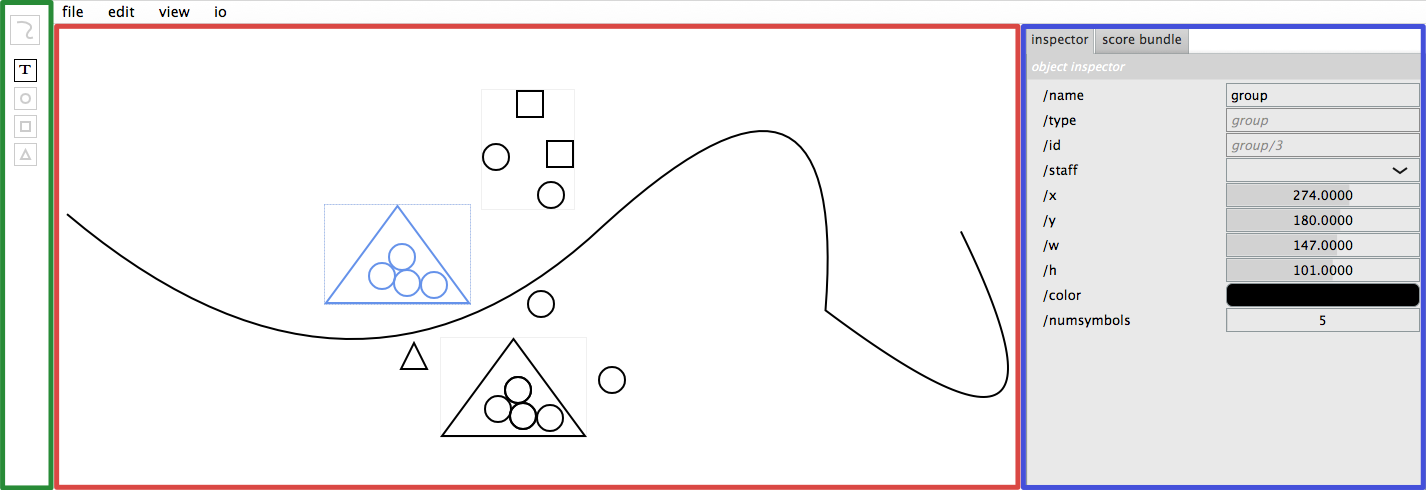
\includegraphics[keepaspectratio=true, width=\textwidth]{LeProjetSymbolist/i/symbolistUIBefore.png}
	\caption{Éditeur graphique de \textit{symbolist}}
	\label{fig:symbolistUIBefore}
	\small
	\it
	En \textcolor{green}{vert}, la palette des symboles disponibles et dessinables sur la partition. En \textcolor{red}{rouge}, la partition, ou l'espace de composition et d'édition des symboles. En \textcolor{blue}{bleu}, l'inspecteur de symboles, qui présente le bundle OSC associé au symbole graphique couramment sélectionné (symbole surligné en bleu dans la partition).
\end{figure}

L'éditeur graphique de \textit{symbolist} permet à l'utilisateur de dessiner directement sur la partition à l'aide de la souris, dans une modèle d'interaction \textit{wysiwyg} (\textit{what you see is what you get}). Dans \textit{symbolist}, la partition fait référence à l'espace graphique où les symboles sont placés et édités par l'utilisateur. 

\paragraph{Concept de staff} De manière sous-jacente, la partition est stockée comme une liste de symboles. Les symboles de la partition qui sont attachés à un référent temporel, un \textit{staff}, se voient attribuer une valeur temporelle de départ et de fin correspondant à leur point de départ et de fin sur l'axe horizontal. Ces symboles sont ordonnancés temporellement dans la liste reflétant la partition.

\paragraph{Environnements d'interactions} De plus, l'éditeur graphique n'est pas le seul moyen d'interagir avec le logiciel \textit{symbolist}. En effet, \textit{symbolist} est également déployer dans une version \textit{objet} pour l'environnement \textit{Max} et l'environnement \textit{OpenMusic}. Dans ces environnements, l'application \textit{symbolist} est représentée comme une boîte, recevant et envoyant des messages à d'autres objets. Les différents messages auxquels répond l'objet \textit{symbolist} dans l'environnement Max sont présentés en figure \ref{fig:symbolistMaxObject}.

\begin{figure}[H]
	\centering
	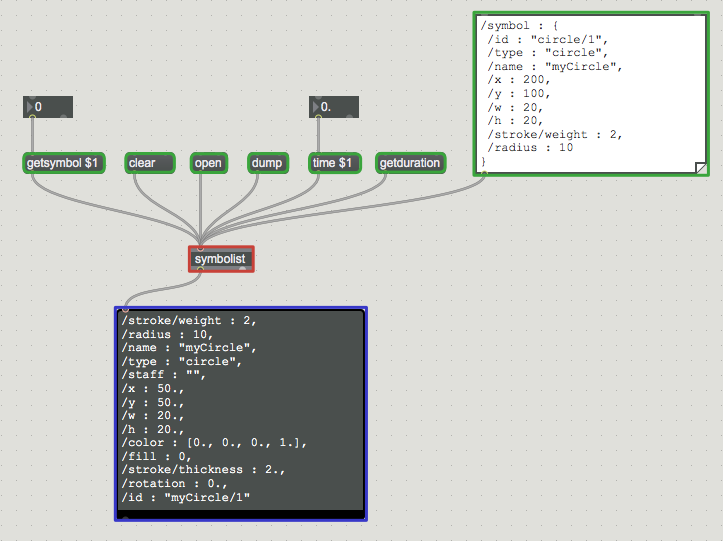
\includegraphics[keepaspectratio=true, width=0.8\textwidth]{LeProjetSymbolist/i/symbolistMaxObject.png}
	\caption{L'objet \textit{symbolist} dans Max}
	\label{fig:symbolistMaxObject}
	\small
	\it
	En \textcolor{red}{rouge}, l'objet \emph{symbolist} représenté, comme tous les objets \emph{Max}, sous forme de boîte. En \textcolor{green}{vert}, les messages pouvant être envoyés à l'objet \emph{symbolist}.
	En \textcolor{blue}{bleu}, un afficheur de bundle OSC, proposé par une librairie indépendante, témoin des messages de sortie générés par l'objet \emph{symbolist}.  
\end{figure}

Les messages\footnote{Dans Max, un message peut être envoyé à un objet via l'objet \textit{message}, qui n'est autre qu'un bouton cliquable avec un label, à connecter à l'entrée d'un receveur.} compris par l'objet \textit{symbolist} permettent de lire et d'écrire des symboles dans la partition.
Comme exemples de messages de lecture, \lstinline|getsymbol n|, lit le \textit{n-ième} symbole de la partition, \lstinline|time t|, lit le contenu de la partition au temps \textit{t}…
Le résultat de la lecture est envoyé sur la sortie de l'objet \textit{symbolist}.

L'écriture de symboles dans la partition se fait par l'envoi de bundles OSC en entrée de l'objet \textit{symbolist} (voir la figure \ref{fig:symbolistMaxObject}, en haut à droite). 
Enfin, l'éditeur graphique peut être lancé par l'envoi du message \lstinline|open|.

\textit{symbolist} est également déployé dans une version objet \textit{OpenMusic}. La figure \ref{fig:symbolistOMObject} montre un exemple de computation de partition avec l'objet \textit{symbolist} (nommé \textit{sym-score}) dans \textit{OpenMusic}.

\begin{figure}[H]
	\centering
	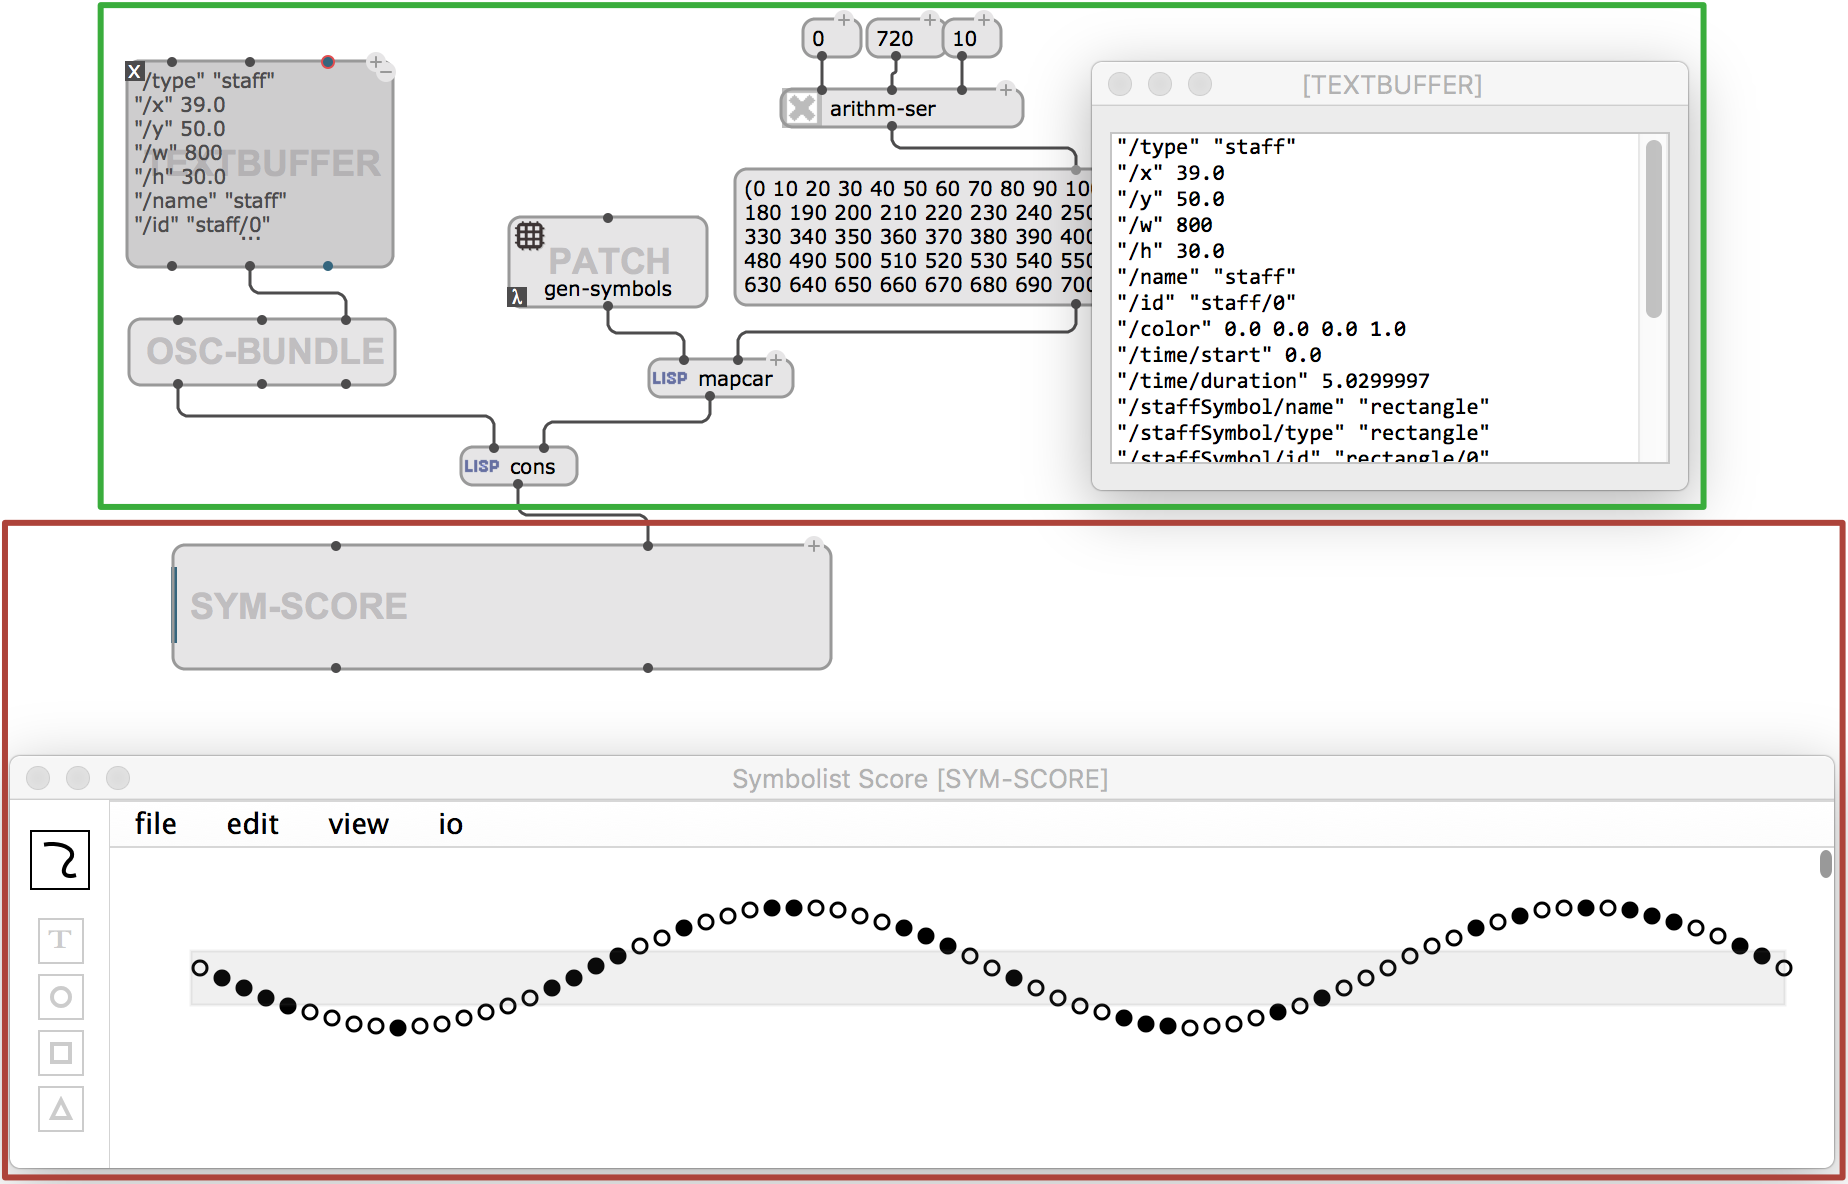
\includegraphics[keepaspectratio=true, width=\textwidth]{LeProjetSymbolist/i/symbolistOMObject.png}
	\caption{L'objet \textit{symbolist} dans OpenMusic}
	\label{fig:symbolistOMObject}
	\small
	\it
	En \textcolor{red}{rouge}, l'objet \emph{symbolist} \og sym-score \fg et l'éditeur graphique associé.
	En \textcolor{green}{vert}, les objets \emph{OpenMusic} servant à la création de bundles OSC envoyés à l'objet \emph{sym-score}.
\end{figure}

L'objet \textit{symbolist} dans sa version \textit{OpenMusic} reçoit des bundles OSC et crée les symboles correspondant dans la partition. Ensuite, le contenu de la partition peut être envoyé sur la sortie, en utilisant la barre de lecture \textit{OpenMusic} (activée par la touche espace).    

\paragraph{Fonctionnalités existantes} Afin de dresser un bilan des fonctionnalités implantées dans \textit{symbolist}, des \textit{user-stories}\footnote{Une \textit{user-story} est une manière d'exprimer une fonctionnalité logiciel, répandue chez les praticiens de la philosophie Agile. Une \textit{user story} prend la forme: \og En tant que tel type d'utilisateur, j'effectue telle action dans tel but \fg. De cette manière, une fonctionnalité est exprimée du point de vue de l'utilisateur, évitant l'écueil d'une formalisation trop technique. } ont été écrites à partir des possibilités du logiciel.
La liste des \textit{user stories} implantées dans \textit{symbolist} au début du stage est la suivante:
\begin{itemize}[label=--]
	\item En tant que compositeur, je dessine des courbes pour créer de nouveaux symboles.
	\item En tant que compositeur, je dessine des formes géométriques pour créer de nouveaux symboles.
	\item En tant que compositeur, j'écris du texte pour créer de nouveaux symboles ou pour annoter ma partition.
	\item En tant que compositeur, j'édite les propriétés d'un symbole existant pour définir sa forme.
	\item En tant que compositeur, je groupe des symboles entre eux pour créer un nouveau symbole.
	\item En tant que compositeur, je transforme un symbole en \textit{staff}, pour définir une référence temporelle dans la partition.
	\item En tant que compositeur, j'associe un symbole à un \textit{staff} pour lui procurer une valeur temporelle.
	\item En tant que compositeur, je peux ajouter un de mes propres symboles à la palette pour le réutiliser ensuite.
	\item En tant que compositeur, je peux annuler/recommencer les actions effectuées sur la partition pour la maintenir dans une état cohérent.
	\item En tant que compositeur, je peux lire le contenu de ma partition à un temps $t$. 
\end{itemize}

Les \textit{user stories} concernant le dessin sur la partition ont été réparties en catégories. En effet, chaque type de symboles est accompagné de problématiques spécifiques, ce qui fait considérer la création de texte, de courbes ou de formes prédéfinies comme des fonctionnalités à part entière.
	
%%%%% CHAPTER "ARCHITECTURE LOGICIELLE DE SYMBOLIST" %%%%%
\chapter{Architecture logicielle de symbolist}
\label{chap:architectureSymbolist}
Ce chapitre expose la contribution majeure de ce stage au développement du logiciel \textit{symbolist}. La première section pose le contexte architectural dans lequel se trouvait \textit{symbolist} au début du stage. La deuxième section souligne les changements  apportés à l'application du point de vue de son architecture logicielle.

	\section{Présentation de l'architecture première}
	\label{sec:architecturePremiere}
	\subsection{Framework de développement pour l'application symbolist}
\label{subsec:frameworkAndTechnologies}
\textit{symbolist} est développé avec le framework \textit{C++} \textit{JUCE} \cite{juce2018}. L'environnement \textit{JUCE} est un standard pour le développement d'applications liées à l'audio. Dans le cas de \textit{symbolist}, \textit{JUCE} a été utilisé pour ses capacités de gestion des bundles OSC et création d'interface graphique. La librairie \textit{odot} a ensuite été préférée pour la gestion des bundles OSC dans \textit{symbolist}. En effet, \textit{odot} augmente les capacités du format OSC, en lui adjoignant par exemple un léger langage de programmation. Aujourd'hui \textit{JUCE} n'est donc plus utilisé dans \textit{symbolist} que pour ses composants graphiques. 

En plus de son framework de développement, l'application \textit{symbolist} est également destinée à être déployée dans les deux environnements que sont \textit{Max} et \textit{OpenMusic}. Aussi, la construction de l'application \textit{symbolist} en tant qu'objet \textit{Max} et \textit{OpenMusic} est détaillée ci-après.

\paragraph{Création d'un objet Max} Max propose une API pour la création de nouveaux objets \cite{maxApi2018}. L'API Max est écrite en \textit{C}, ainsi que doivent l'être les objets créés par les utilisateurs pour étendre le système.
Ces objets sont appelés des \textit{externals} dans Max.
Ils doivent posséder une certaine structure pour pouvoir être compilé et utilisé par la suite:
\begin{itemize}[label=--]
	\item Le fichier de définition de l'external doit inclure le header \textit{ext.h} à la première ligne.
	\item Le nouvel objet défini doit être déclaré comme une structure \textit{C} avec un premier champ de type spécial.
	\item Une méthode de création et de libération de l'objet doivent être définies, ainsi qu'une méthode pour chaque message que peut recevoir l'objet.
	\item Ces méthodes sont liées à l'objet au sein de la procédure \lstinline|ext_main| qui fait office de procédure d'initialisation. De fait, \lstinline|ext_main| est appelée lorsque l'objet cible est appelé dans un patch Max, c'est à dire lorsque son nom est tapé dans une boîte.
\end{itemize}

L'application \textit{symbolist} étant implémentée en \textit{C++}, une API équivalente en \textit{C} a été écrite afin de pouvoir communiquer avec \textit{Max} et \textit{OpenMusic}.
Les méthodes fournies par l'API \textit{C} \textit{symbolist} sont présentées en annexe , page .
\todo[inline]{Ajouter l'API C symbolist en annexe}  

\paragraph{Création d'un objet OpenMusic} \textit{OpenMusic} pouvant être vu comme une surcouche graphique du langage \textit{Common Lisp} et de son système objet \textit{CLOS} \cite{bresson2009}, la création de nouveaux objets \textit{OpenMusic} est équivalent à la définition d'une nouvelle classe \textit{Lisp}.
Par exemple, l'objet \textit{symbolist} dans \textit{OpenMusic} est définie comme une classe possédant deux attributs: l'attribut \textit{symbols}, une liste de bundles OSC représentant la partition, et l'attribut \textit{palette-symbols}, une autre liste de bundles OSC représentant la palette des symboles disponibles.  
De fait, la boîte représentant l'objet \textit{symbolist} dans \textit{OpenMusic} possède trois points d'entrée et de sortie. Le premier point d'entrée correspond à la définition par copie d'un objet \textit{symbolist} par un autre objet \textit{symbolist}; le point d'entrée est dénommé \textit{self}. Les deux autres points d'entrées correspondent aux attributs de l'objet \textit{symbolist}, \textit{symbols} et \textit{palette-symbols}.
Les mêmes points se retrouvent symétriquement définis en sortie.

Un objet \textit{OpenMusic} peut également être muni d'un éditeur, c'est à dire une fenêtre graphique apparaissant lors d'un double-clic sur l'objet. L'éditeur associé à un objet \textit{OpenMusic} est défini par une classe \textit{Lisp} étendant la classe \textit{OMEditor}. 
Dans le cas de l'objet \textit{symbolist}, son éditeur fait la liaison avec l'API \textit{C} permettant de contrôler avec l'application \textit{symbolist} et son interface.
 
\subsection{Architecture de l'application symbolist}
\label{subsec:architectureBefore}
Le framework \textit{JUCE}, utilisé pour développer l'application \textit{symbolist}, n'impose pas d'architecture logicielle. Aussi, les applications développées avec ce framework définissent chacune leurs propres structures.
L'architecture logicielle de \textit{symbolist} n'est pas clairement définie au début de ce stage, néanmoins trois parties peuvent être distinguées dans le code source. 

Une première partie est centrée autour de la classe \textit{SymbolistHandler}. Cette classe permet l'accès depuis l'extérieur à l'application \textit{symbolist}. A savoir, l'API \textit{C} permettant à \textit{Max} et \textit{OpenMusic} de communiquer avec \textit{symbolist} appelle les méthodes de la classe \textit{SymbolistHandler} pour pouvoir interagir avec le reste de l'application.

Une deuxième partie correspond aux composants graphiques construisant l'interface de \textit{symbolist}. La fenêtre principale de l'application \textit{symbolist} est représentée par la classe \textit{SymbolistMainComponent}. Cette partie comprend également toute la hiérarchie des composants graphiques représentant les symboles de la partition.

La troisième partie de l'application regroupe les classes du \og cœur métier \fg, représentant la partition et la palette du compositeur. 
S'y trouvent les classes implémentant la structure des bundles OSC, où plus précisément des bundles \textit{odot}, qui définissent le format de données sous-jacent des symboles de la partition.
Pour décrire les symboles de la partition, l'application \textit{symbolist} possède une unique classe \textit{Symbol} (qui hérite de la classe \textit{OdotBundle}). De fait, chaque symbole de la partition, qu'il soit un rond, un carré, une note de musique, ou du texte, est représentée par une instance de la classe \textit{Symbol}. Les spécificités d'un symbole ne sont pas explicitées par sa classe d'appartenance; 
à savoir, le modèle ne prévoit pas de classes \textit{Circle}, \textit{Square} ou \textit{MusicNote}.
En effet, la philosophie de \textit{symbolist} est de conserver l'information des symboles dans les bundles OSC sous-jacents afin de pouvoir distribuer plus facilement les données de la partition.
Les classes du cœur métier incluent également toute la logique d'ordonnancement temporel des symboles associés à un \textit{staff}.
Le diagramme de classes détaillée du cœur métier de l'application \textit{symbolist} est présenté en annexe \ref{sec:symbolistModelClassDiagram}, page~\pageref{sec:symbolistModelClassDiagram}.

\paragraph{Problématiques architecturales} Plusieurs aspects posent un problème dans l'architecture de l'application \textit{symbolist} telle qu'elle se trouve au début du stage.

Premièrement, de la description des composantes de l'application \textit{symbolist} se dégage aisément une architecture de type \textit{modèle-vue-contrôleur}. Cependant, les interactions entre composantes et le rôle de chacune d'elles ne sont pas biens définis. Par exemple, la création de symboles dans \textit{symbolist}, de fait l'écriture dans le \textit{modèle}, est trop souvent réalisée par les composants graphiques du système, ce qui est contraire à l'architecture \textit{MVC}. 

Deuxièmement, même si le modèle de l'application \textit{symbolist} place les symboles de la partition à un même niveau dans la hiérarchie des classes (à savoir, il n'existe qu'une seule classe \textit{Symbol}), les composants graphiques sont eux le reflet de la structure de la partition.
C'est à dire, chaque type de composant graphique est représenté par une classe: par exemple, les cercles sont représentés par la classe \textit{CircleComponent}, les rectangles par la classe \textit{RectangleComponent}…
Aussi, comme les symboles de la partition peuvent être groupés afin de créer de nouveaux symboles, le design pattern \textit{Composite} est approprié à la hiérarchie des composants graphiques. 
Or, au début de ce stage, le design pattern \textit{Composite} n'est pas correctement appliqué. 

Troisièmement, la classe \textit{SymbolistHandler}, qui est directement liée à l'API \textit{C} rendant \textit{symbolist} utilisable par d'autres programmes, s'occupe de toutes les interactions avec les vues de l'interface: la palette, la partition, l'inspecteur… Aussi, la classe \textit{SymbolistHandler} est trop encombrée, et les interactions avec des vues spécifiques mériteraient d'être gérées par des contrôleurs spécifiques.


	\section{Restructuration de l'application symbolist}
	\label{sec:restructurationSymbolist}
	L'un des objectifs du stage était d'étudier et structurer l'application \textit{symbolist} en lui appliquant le design pattern \textit{Model-View-Controller}, avec quelques adaptations de circonstances.
La présente section rend compte des changements appliqués à l'architecture de \textit{symbolist}, dans une démarche de stabilisation structurelle.

\subsection{Application du design pattern Model-View-Controller}
\label{subsec:applicationDuMVC}
Le \og paradigme \fg \textit{MVC} est une manière de structurer une application qui relève d'une séparation en trois parties : le modèle, la vue et le contrôleur \cite{krasner1988}. Le but de la manœuvre est de confiner les préoccupations fonctionnelles de chaque partie, et de définir leurs interactions afin de rendre plus intuitive la marche à suivre par le programmeur lors de l'implémentation d'une nouvelle fonctionnalité.

\paragraph{Implémentation de la structure élémentaire.} Le framework \textit{JUCE} ne disposant pas de classes abstraites décrivant les parties du \textit{MVC}, la structure sous-jacente de l'architecture a été implémentée en \textit{C++}. La figure \ref{fig:mvcApi} décrit le diagramme de classes définissant les concepts élémentaires de l'architecture \textit{MVC}. Ce diagramme a servi de base pour l'implémentation de la structure \textit{MVC} dans \textit{symbolist}.

\begin{figure}[H]
	\centering
	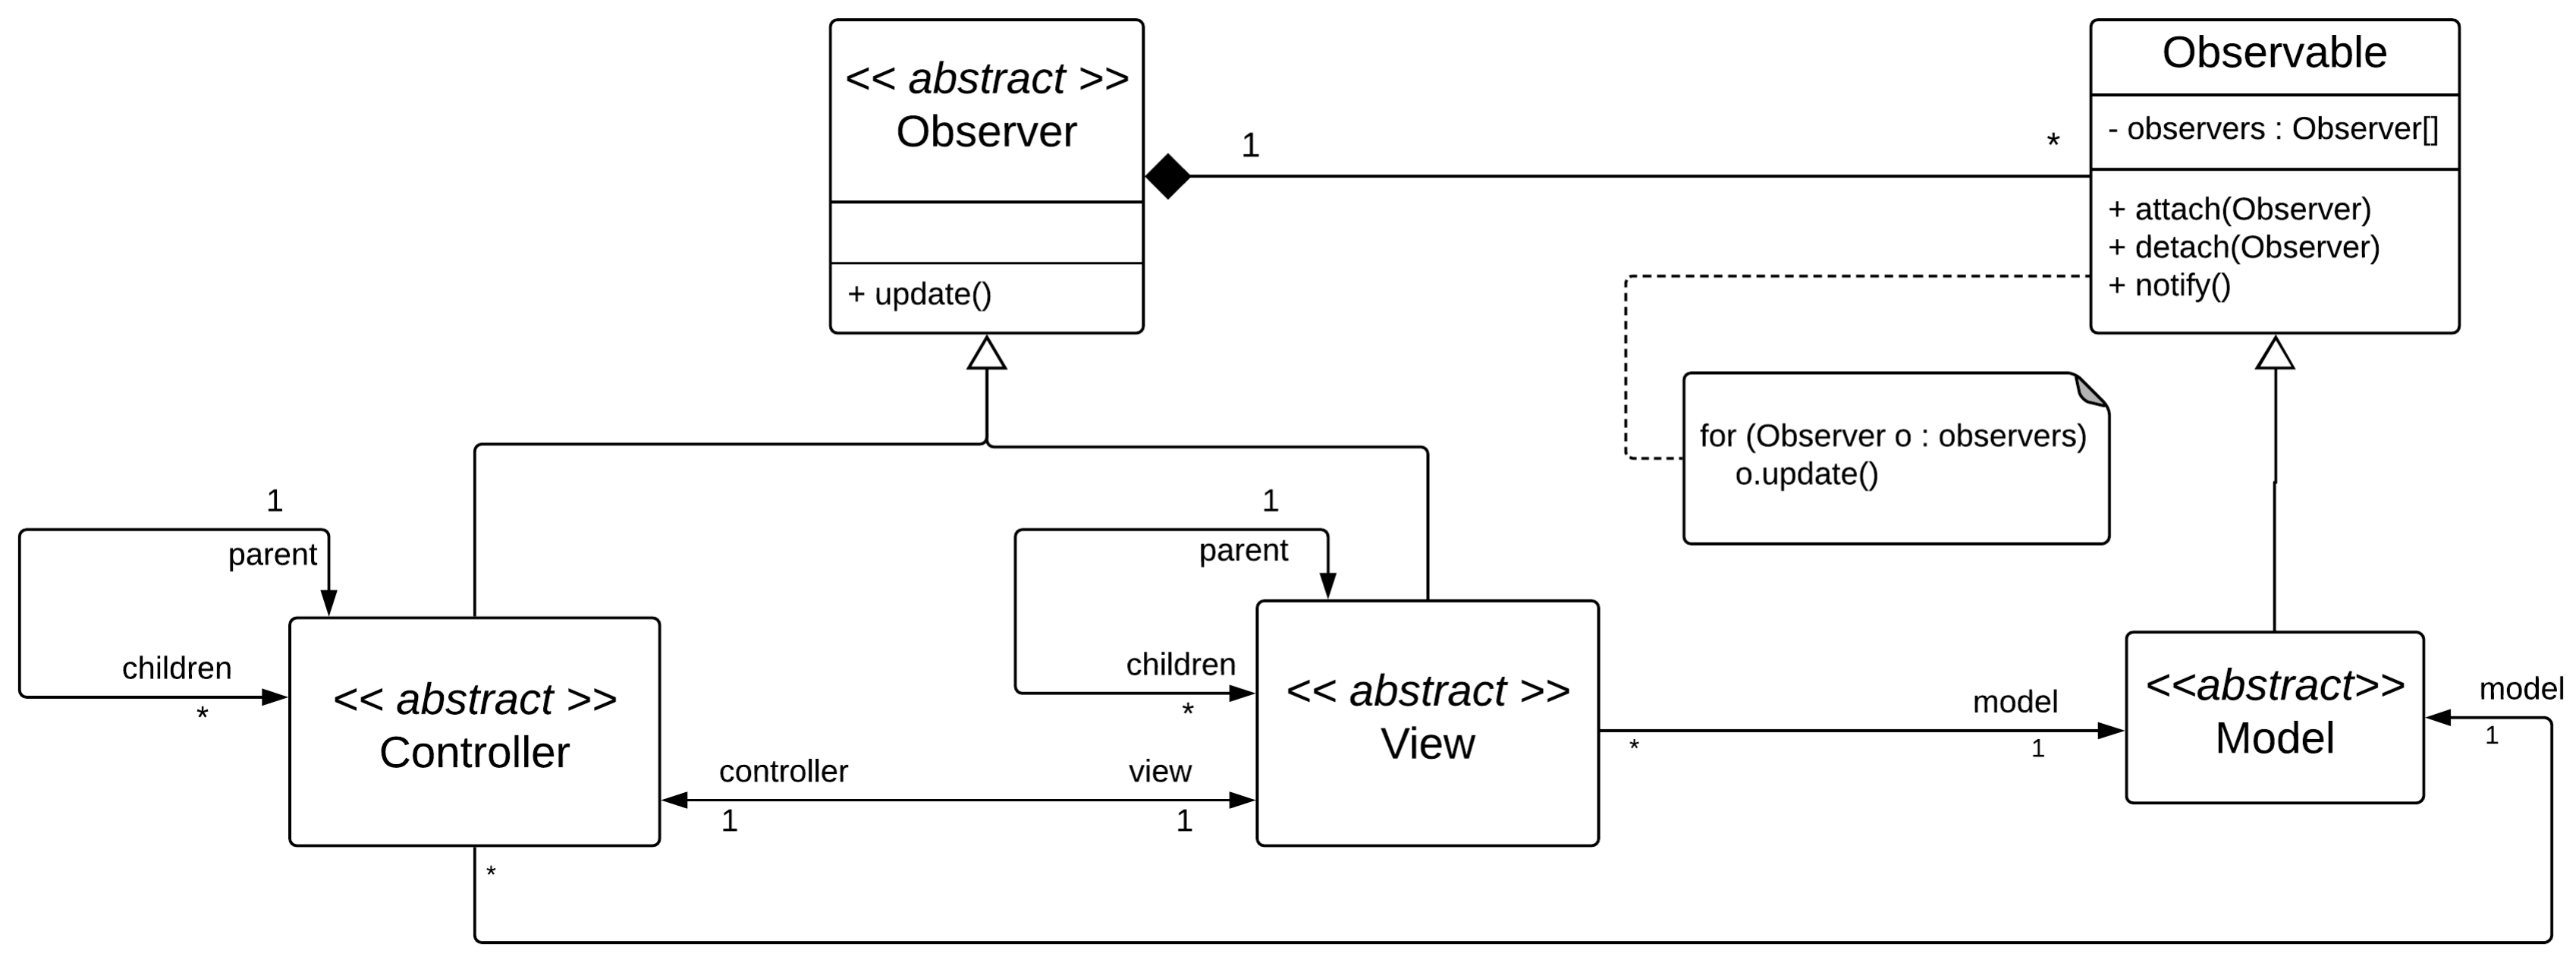
\includegraphics[keepaspectratio=true, width=\textwidth]{ArchitectureLogicielle/i/mvcApi.png}
	\caption{Diagramme de classes pour une API MVC}
	\label{fig:mvcApi}
	\small
	\it
\end{figure}

Premièrement, dans le paradigme \textit{MVC}, les vues et les contrôleurs de l'application sont informés des changements survenus dans le modèle par le biais d'un système de souscription, plus connu sous le nom de design pattern \textit{Observer}. Comme présenté en figure \ref{fig:mvcApi}, les contrôleurs et vues du système héritent de la classe \textit{Observer} la méthode \textit{update}, qui est appelée par l'objet observé - ici le modèle héritant de la classe \textit{Observable} - lorsque celui-ci est modifié.
Toutes actions d'écriture dans le modèle déclenche l'envoi du message \textit{update} aux observateurs. Par exemple, dans le cas de \textit{symbolist}, la création ou la délétion d'un symbole dans la partition ou dans la palette donne lieu à l'envoi du message \textit{update}.
La réaction des observateurs à la réception du message \textit{update} doit être définie dans les sous-classes de la classe \textit{Observer}. Aussi, les classes \textit{Controller} et \textit{View} décrivant des comportements génériques pour les vues et contrôleurs d'une application, aucune implémentation de la méthode \textit{update} n'y est définie, d'où leur statut de classe abstraite.

Deuxièmement, les relations entre les classes \textit{Controller}, \textit{View} et \textit{Model} sont définis comme présentées en figure \ref{fig:mvcApi}. Un contrôleur et une vue sont associés par couple; ils se référencent mutuellement. Chaque vue et chaque contrôleur d'une application connaissent le modèle auquel ils sont rattachés; ils en ont un accès direct. Cependant, le modèle d'une application ne connaît pas directement les contrôleurs et les vues qui l'observent; il les contacte par le biais du message1 \textit{update} exclusivement.

Troisièmement, l'interface d'une application pouvant être découpée en sous-vues, un système de hiérarchie a été mis en place, représentée par les relations réflexives des classes \textit{View} et \textit{Controller}. En effet, dans le paradigme \textit{MVC}, la hiérarchie des vues est répliquée pour les contrôleurs \cite{krasner1988}. Aussi, une application sera composée d'une vue \textit{racine}, la fenêtre du programme, laquelle sera divisée en sous-vues. Parallèlement, cette application possèdera un contrôleur \textit{racine} associé à la vue \textit{racine}, qui sera le parent de sous-contrôleurs associés à chaque sous-vues du programme.

\paragraph{Structures préexistantes} La structure du programme \textit{symbolist} avant remaniement a été présentée succinctement en section \ref{subsec:architectureBefore}. Le modèle de l'application étant détaillé en annexe \ref{sec:symbolistModelClassDiagram}, page~\pageref{sec:symbolistModelClassDiagram}, seules les parties vue et contrôleur de l'application seront présentées ici.
La figure \ref{fig:controllerDiagramBefore} décrit le diagramme de classes \og côté contrôleur \fg, au début du stage.

\begin{figure}[H]
	\centering
	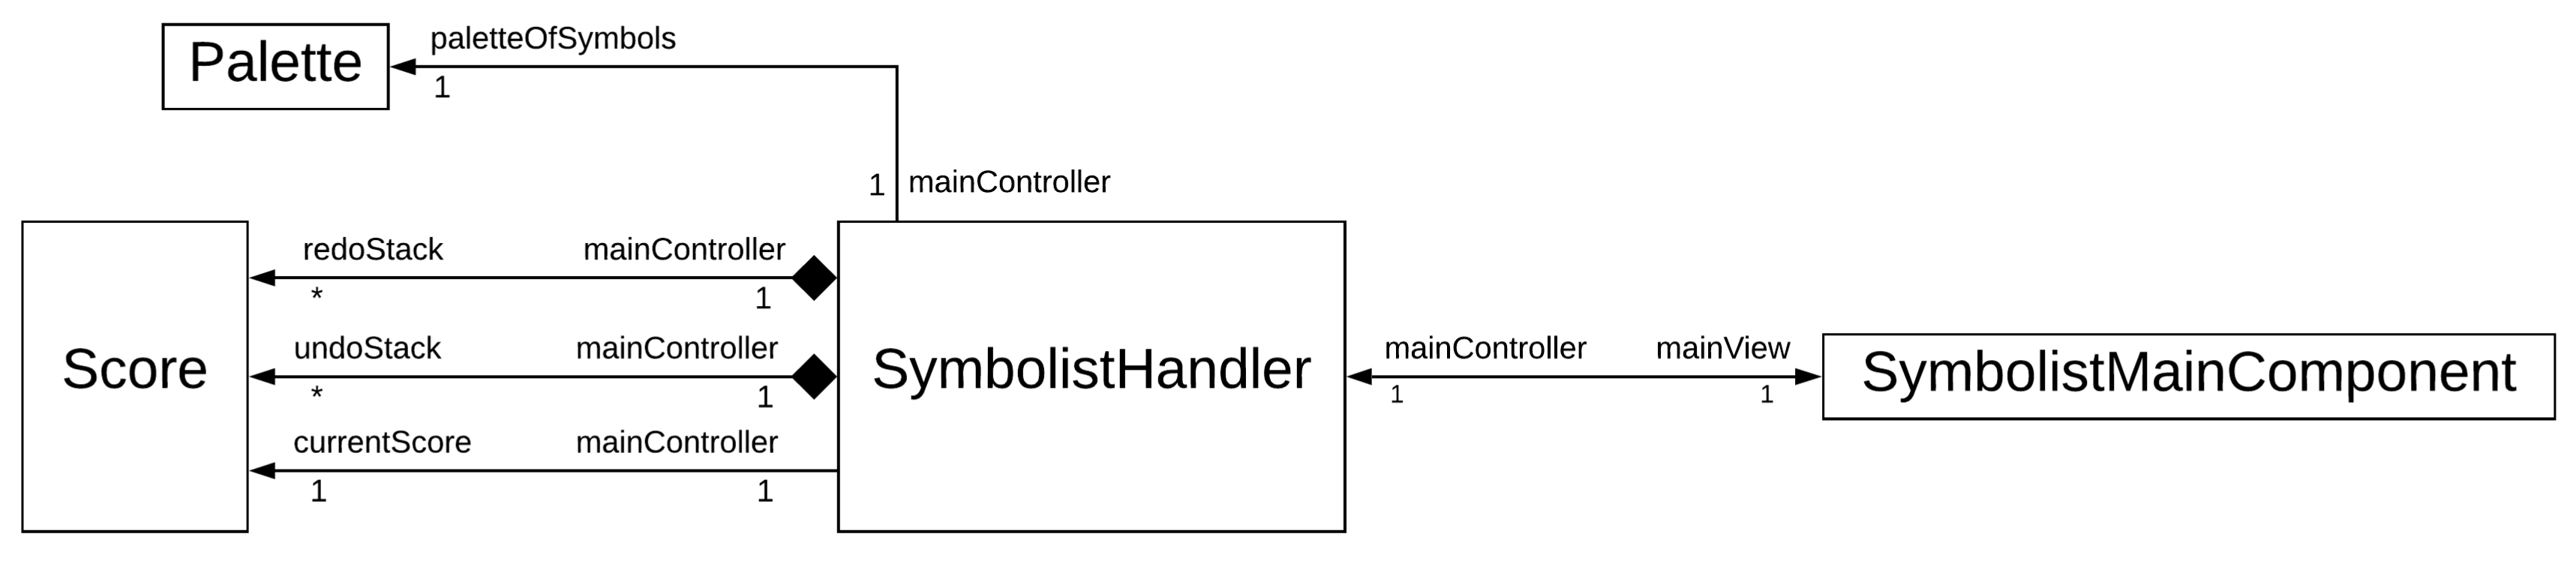
\includegraphics[keepaspectratio=true, width=\textwidth]{ArchitectureLogicielle/i/controllerDiagramBefore.png}
	\caption{Diagramme de classes pour la partie contrôleur avant restructuration}
	\label{fig:controllerDiagramBefore}
	\small
	\it
\end{figure}

Avant restructuration, la classe \textit{SymbolistHandler} est la seule à référencer directement le modèle, représenté par les classes \textit{Palette} et \textit{Score}. Les vues de l'application doivent systématiquement passer par la classe \textit{SymbolistHandler} afin d'accéder aux données du modèle. Préliminairement à la restructuration, le couple contrôleur principal-vue principale est déjà réifié par la liaison entre la classe \textit{SymbolistHandler} et \textit{SymbolistMainComponent}.

La figure \ref{fig:viewDiagramBefore} expose le diagramme de classes simplifié de la partie \og vue \fg de l'application \textit{symbolist} au début du stage.

\begin{figure}[H]
	\centering
	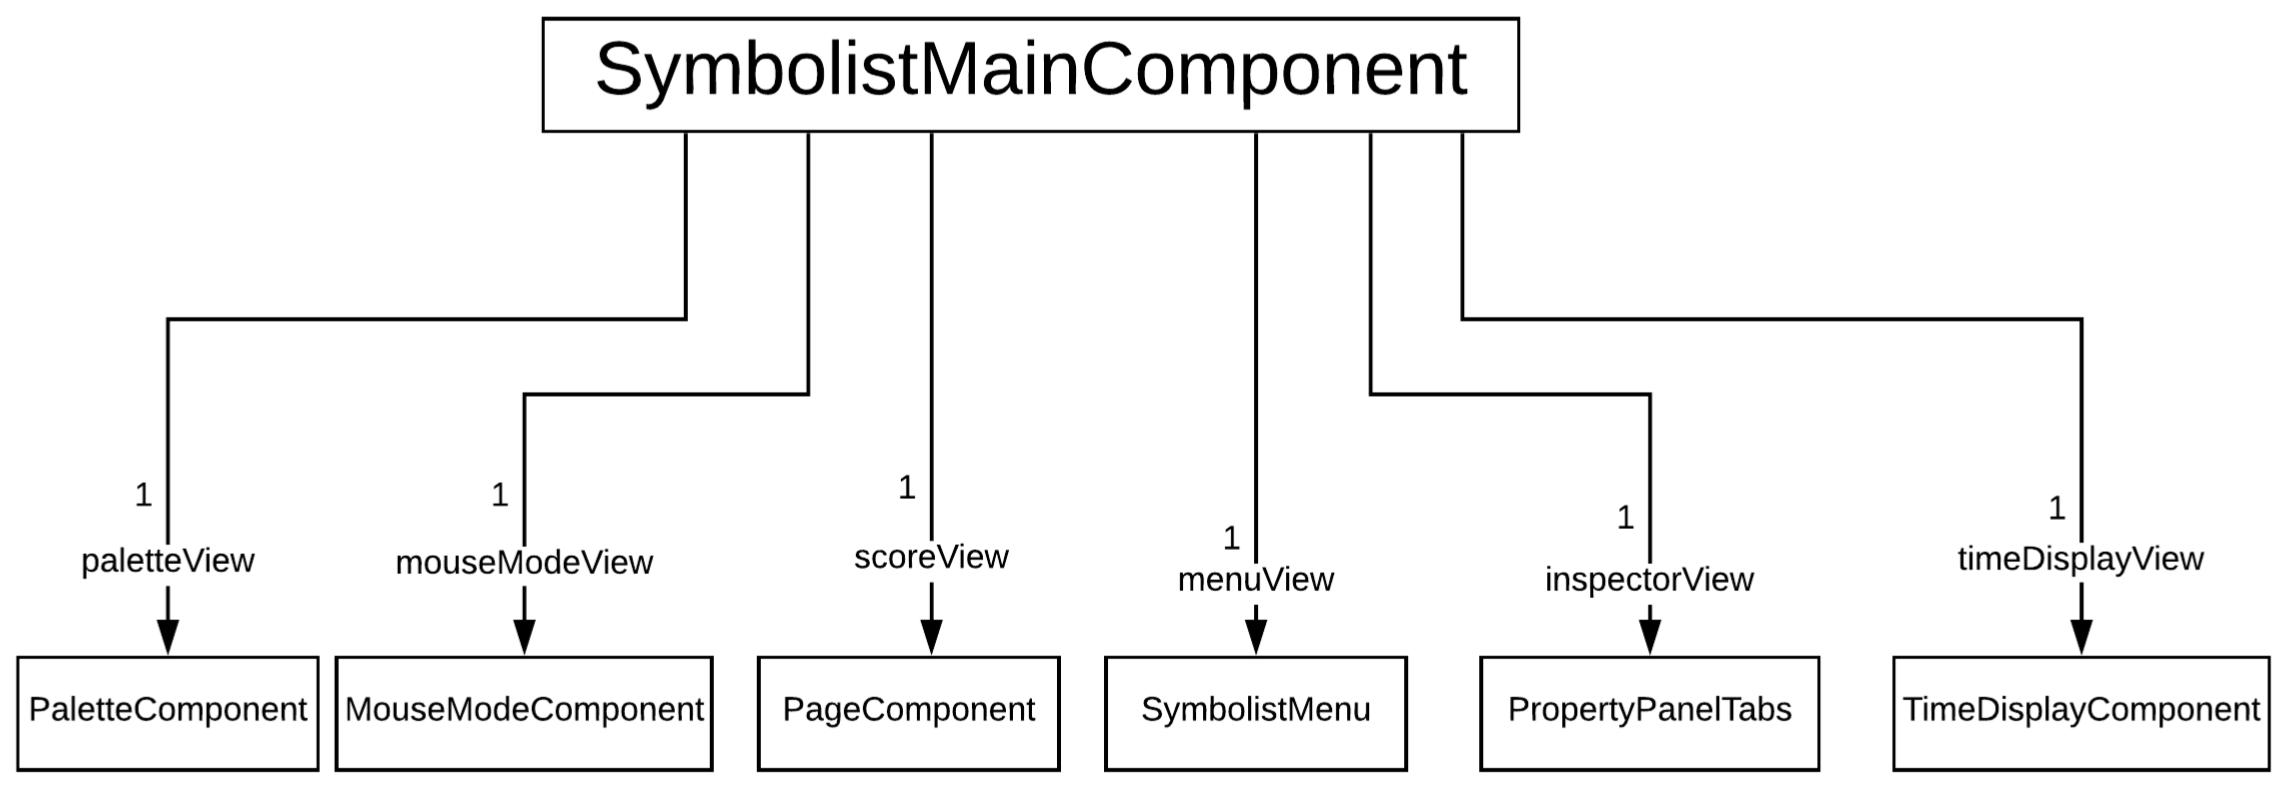
\includegraphics[keepaspectratio=true, width=0.8\textwidth]{ArchitectureLogicielle/i/viewDiagramBefore.png}
	\caption{Diagramme de classes pour la partie vue avant restructuration}
	\label{fig:viewDiagramBefore}
	\small
	\it
\end{figure}

La classe \textit{SymbolistMainComponent} représente la vue principale de l'application \textit{symbolist}. Elle référence toutes les sous-vues de l'application, comme la vue représentant la palette des symboles utilisables (\textit{paletteView}) et la vue décrivant la partition (\textit{scoreView}).

\paragraph{Implémentation du design pattern MVC} La première démarche de restructuration a été de faire hériter les classes de l'application \textit{symbolist} des classes de l'API \textit{MVC} présentées en figure \ref{fig:mvcApi}.
La classe \textit{SymbolistHandler} a donc hérité de la classe \textit{Controller} et la classe \textit{SymbolistMainComponent} et ses sous-vues ont hérité de la classe \textit{View}.
Afin de lier chaque instance de \textit{View} et \textit{Controller} à une instance du modèle, une classe \textit{SymbolistModel} a été créée, référençant la partition et la palette de l'application.
L'encapsulation des classes \textit{Score} et \textit{Palette} dans \textit{SymbolistModel} permet d'envoyer plus facilement le message \textit{update} aux observateurs du modèle à chaque fois qu'une action de modification est entreprise.

Ensuite, un contrôleur a été créé et couplé avec chacune des sous-vues de l'application afin de gérer plus localement les interactions avec l'utilisateur.  
Une fois la structure globale de l'application établie, le travail a consisté à s'assurer que les éléments de l'architecture MVC se comportent correctement, depuis la captation d'une action utilisateur jusqu'à sa répercussion sur l'interface graphique de \textit{symbolist}.
Pour plus d'informations sur la structure finale du programme, le diagramme de classes décrivant la nouvelle architecture de l'application \textit{symbolist} est présentée en annexe \ref{sec:symbolistFinalStructure}, page~\pageref{sec:symbolistFinalStructure}.

\subsection{Restructuration de la hiérarchie des composants graphiques}
\label{susec:graphicComponentRestruct}
Une des volontés de \textit{symbolist} est de conserver l'information descriptive des symboles de la partition dans le canevas d'un bundle OSC. De fait, le modèle de l'application \textit{symbolist} ne possède qu'une seule classe \textit{Symbol} pour décrire les éléments d'une partition.
La structure hiérarchique (encapsulation de symboles dans d'autres symboles) qui peut être celle d'une partition \textit{symbolist} se trouve cachée dans les bundles OSC du modèle.
Aussi, ce sont aux classes représentant graphiquement les symboles de refléter cette structure.
De même, si les symboles du modèle participent d'une seule et même classe \textit{Symbol}, il possède cependant un attribut \textit{type} qui va orienté le contenu des messages OSC composant le bundle les décrivant.
Par exemple, un symbole de type \textit{circle} possédera l'attribut \textit{radius} dans son bundle, alors qu'un symbole de type \textit{rectangle} possèdera un attribut \textit{width} et \textit{height}.
Au même titre que chaque type de symbole oriente la construction du bundle sous-jacent, les classes à composants graphiques décrivant la partition \textit{symbolist} doivent être spécialisées pour refléter chacun des types de symboles.
Au début de ce stage, la hiérarchie des composants graphiques est déjà établie. La figure \ref{fig:graphicCompBefore} présente la diagramme de classes, avant restructuration, des composants décrivant une partition \textit{symbolist}.

\begin{figure}[H]
	\centering
	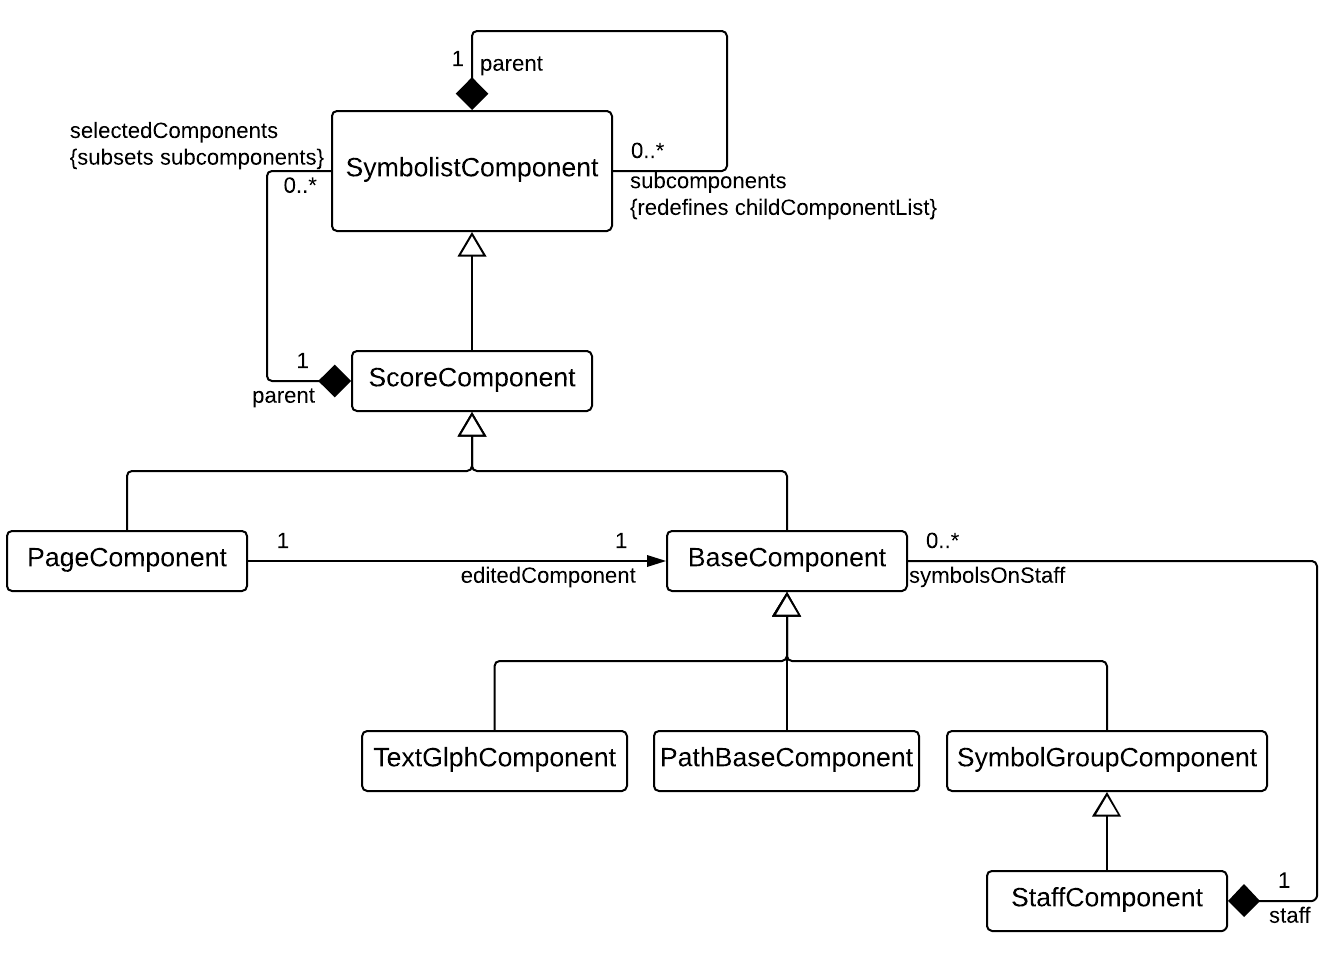
\includegraphics[keepaspectratio=true, width=0.8\textwidth]{ArchitectureLogicielle/i/graphicCompBefore.png}
	\caption{Diagramme de classes des composants graphiques d'une partition symbolist avant restructuration}
	\label{fig:graphicCompBefore}
	\small
	\it
	La classe \emph{SymbolistComponent} est la classe mère de tous les composants graphiques de l'application \emph{symbolist}. Elle contient des méthodes de récupération de référence vers les vues principales, comme \emph{SymbolistMainComponent}, et vers la classe \emph{SymbolistHandler}.
	La classe \emph{ScoreComponent} est la classe mère de tous les composants graphiques appartenant à une partition \emph{symbolist}.
	La classe \emph{PageComponent} correspond à la vue de la partition, elle est associée à un \emph{PageController}.
	La classe \emph{BaseComponent} et ses sous-classes décrivent plus précisément chaque type de symbole graphique de la partition, qu'ils soient dessinés par tracé (\emph{PathBaseComponent}), qu'ils représentent du texte (\emph{TextGlphComponent}) ou qu'ils soient une composition de symboles
	(SymbolGroupComponent).
\end{figure}

La construction des classes comme présentéee en figure \ref{fig:graphicCompBefore} souffre de faiblesses structurelles. Par exemple, le design pattern \textit{Composite}, qui serait prescrit pour représenter la hiérarchie des composants graphiques, n'est que partiellement appliqué.
La classe \textit{PageComponent}, qui représente la partition et qui est donc un ultime groupe de symboles, n'est pas regroupée avec la classe \textit{SymbolGroupComponent} sous une même égide d'éléments composites.
De plus, la classe \textit{BaseComponent}, dont héritent tous les composants graphiques présents dans la partition, ne suffit pas à clairement différencier les éléments composites des éléments simples.

La structure globale des composants graphiques a été remaniée en conséquence. Le résultat du remaniement est présenté par le diagramme de classes de la figure \ref{fig:graphicCompAfter}.

\begin{figure}[H]
	\centering
	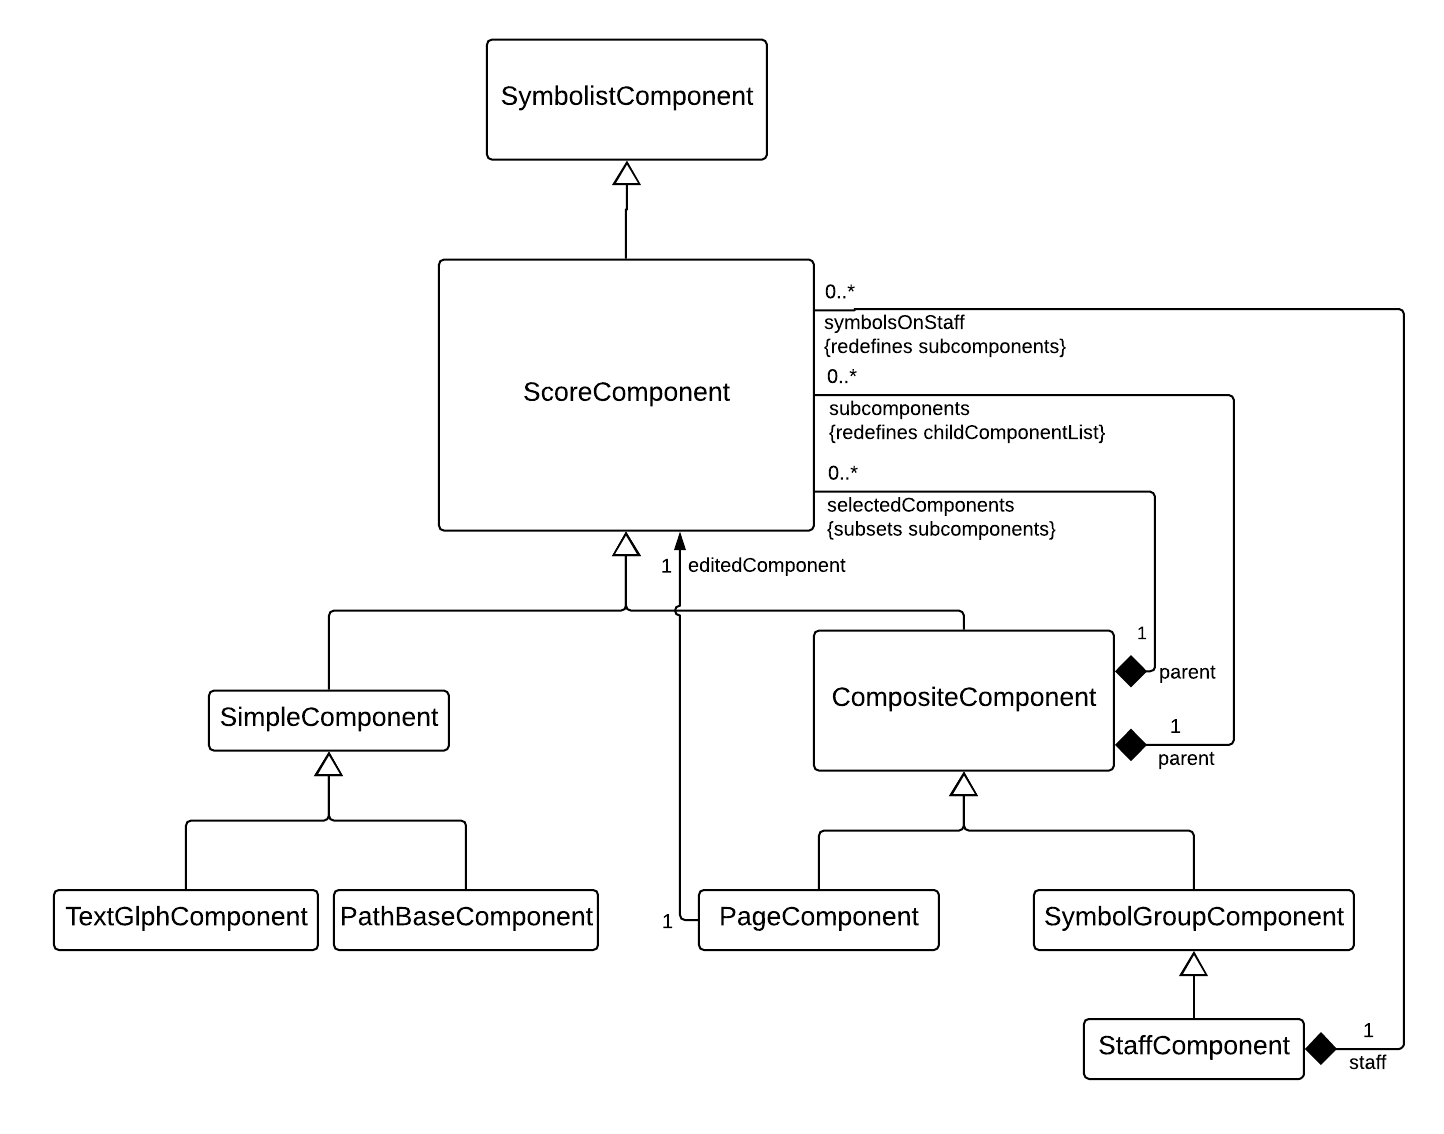
\includegraphics[keepaspectratio=true, width=0.8\textwidth]{ArchitectureLogicielle/i/graphicCompAfter.png}
	\caption{Diagramme de classes des composants graphiques d'une partition symbolist après restructuration}
	\label{fig:graphicCompAfter}
	\small
	\it
\end{figure}

Deux nouvelles classes ont donc été crées pour appliquer pleinement le pattern \textit{Composite}: \textit{SimpleComponent} et \textit{CompositeComponent}\footnote{\textit{SymbolGroupComponent} aurait pu généraliser le concept d'élément composite, cependant cette classe étant concrète, une nouvelle classe abstraite \textit{CompositeComponent} a été créée.}. La classe \textit{PageComponent} a été déplacée pour hériter de la classe \textit{CompositeComponent}.
De même, les relations \textit{subcomponents}, \textit{symbolsOnStaff} et \textit{selectedComponents}, permettant la composition et la sélection de symboles dans les éléments composites ont migrés à leur juste place entre la classe \textit{CompositeComponent} et \textit{ScoreComponent}.



%%%%% CHAPTER "VERS UN MODELE ABSTRAIT ET EXECUTABLE POUR LA NOTATION MUSICALE" %%%%%
\chapter{Vers un modèle abstrait et exécutable pour la notation musicale}
\label{chap:modeleDeNotation}
	
	\todo[inline]{Intro, présentation de la contribution à symbolist dans une optique de renouvellement du modèle de notation}
	\section{Notation exécutable}
	\label{sec:notationExecutable}
	La notion de notation musicale exécutable est intimement lié au format de partition numérique. Deux sens peuvent être prêtés au terme de notation musicale exécutable. 
Premièrement, une partition est exécutable si elle peut contribuer à la production d'un résultat musical, ou sonore, lors de sa lecture par un ordinateur. Il existe alors une dépendance (\textit{mapping}) entre les paramètres graphiques de la partition et les paramètres de production du son. Cette dépendance permet aussi bien à une partition de piloter un synthétiseur que de transcrire graphiquement les variations dans le jeu musical de ce même synthétiseur.

Deuxièmement, l'exécutabilité d'une notation peut également provenir des actions de modification de son propre contenu (modification graphique ou sur les données envoyées) lors de sa lecture temporelle. Par exemple, un  symbole placé sur une partition peut être un déclencheur d'évènement, qui à sa lecture entraîne la modification de la partition (création, modification, suppression d'autres symboles…). Cette logique de fonctionnement est celle utilisée par INScore pour la création de partitions \textit{interactives} \cite{fober2017}.
Aussi, cette idée d'encapsulation d'intelligence programmationnelle dans un symbole est atteinte dans \textit{symbolist} grâce à l'utilisation de la librairie \textit{odot} et son système d'expressions \cite{maccallum2011}.

\subsection{La librairie odot}
\label{subsec:odotLibrary}
La librairie \textit{odot}, développée au laboratoire CNMAT de l'Université de Berkeley, offre une implémentation en langage C du format OSC augmenté de certaines possibilités. Notamment, le \og format \fg \textit{odot} multiplie les types de données pouvant être contenus dans un message OSC. Par exemple, un bundle OSC peut être stocké dans un message, rendant possible l'imbrication de bundles (comme au format JSON). 
La librairie \textit{odot} a été encapsulé en C++ afin d'être intégré à \textit{symbolist}. Comme évoqué plus haut, \textit{odot} met à disposition un langage de programmation, appelé \textit{o.expr}, qui permet d'appliquer des expressions \og à la C \fg à des bundles OSC. \textit{o.expr} permet d'ajouter des messages à un bundle OSC ou de modifier la valeur d'un message préexistant. La figure \ref{fig:applyOdotExpr} donne un exemple de bundle OSC avant et après l'application d'une expression \textit{odot}.

\begin{figure}[H]
	\centering
	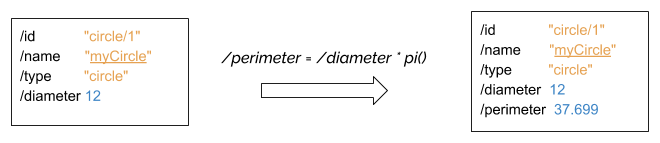
\includegraphics[keepaspectratio=true, width=\textwidth]{ModeleDeNotation/i/applyOdotExpr.png}
	\caption{Application d'une expression odot à un bundle OSC}
	\label{fig:applyOdotExpr}
	\small
	\textit{A gauche, le bundle OSC avant l'application de l'expression \emph{/perimeter = /diameter * pi()}. A droite, le bundle OSC résultant.}
\end{figure}

Le langage d'expressions \textit{odot} met à disposition de l'utilisateur un certain nombre de primitives: des fonctions pour le calcul mathématique (\texttt{pi()}, \texttt{e()}, \texttt{sum()}, \texttt{product()}...), des fonctions pour la recherche et le listing d'adresses et de valeurs de messages OSC (\texttt{getadresses()}, \texttt{getvalues()}...), mais aussi la possibilité de définir des lambda fonctions et des fonctions de mapping (\texttt{lambda()}, \texttt{map()}...).

Une des contributions de ce stage a été de rendre possible l'application d'expressions \textit{odot} à un symbole (qui est sous-jacemment un bundle OSC) dans une partition \textit{symbolist}. L'application d'une expression \textit{odot} à un symbole passe par l'inspecteur de l'interface \textit{symbolist}, comme montré en figure.

\todo[inline]{Ajouter une figure avec l'inspecteur symbolist et l'evaluation odot}

Par convention, l'expression \textit{odot} à appliquer à un symbole est contenue dans le message OSC d'adresse \texttt{/expr}.
Aussi, lors de la lecture d'une partition \textit{symbolist}, chaque symbole envoyé en sortie est évalué, c'est à dire l'expression \textit{odot} contenue dans \texttt{/expr} -  sous réserve de son existence - est appliquée au symbole.
De cette manière, un nombre illimité de nouvelles informations peuvent être générées lors de la lecture d'une partition \textit{symbolist}. La figure montre comment une expression \textit{odot} peut être utilisée pour créer d'autres symboles, notamment grâce aux objets \textit{Max} de la librairie \textit{odot}.

\todo[inline]{Ajouter une figure avec un exemple de création de nouveau bundle en bouclant sur l'objet symbolist}

\subsection{La partition comme pilote des paramètres du son} 
\label{subsec:partitionPiloteSon}
Une partition peut-être vue comme une suite d'instructions (d'évènements) pour exécuter une pièce musicale \cite{bosseur2005}. Contrairement aux interactions traditionnelles où la partition est décodée par l'interprète humain pour produire de la musique, dans un environnement numérique, la partition contrôle un ou plusieurs processus informatiques (qui deviennent à leur tour des interprètes) dans le but de produire un résultat musical (ou multimédia).
Dans \textit{symbolist}, chaque symbole de la partition est décrit par un bundle OSC (voir section \ref{sec:geneseSymbolist}), qui liste, dans un format standardisé (couples adresse-valeur), les attributs du symbole associé.
Le format OSC étant standard en informatique musicale, \textit{symbolist} en tire avantage pour pouvoir communiquer des informations contenues dans une partition à d'autres processus informatiques (application, objets, composants logiciels…), dans le but de contrôler leurs paramètres d'entrées.
Alors, la question suivante se pose: comment lier, dans un paradigme de communication OSC, les attributs d'un symbole aux paramètres d'entrée d'un processus informatique?

Une exemple simple peut être pris pour illustré le principe de connexion entre attributs de symbole et paramètres de processus. La figure \ref{fig:linkingParameters} présente un exemple de partition créée avec \textit{symbolist} qui a pour but de contrôler la hauteur du son (en Hertz) produit par un synthétiseur.

\begin{figure}[H]
	\centering
	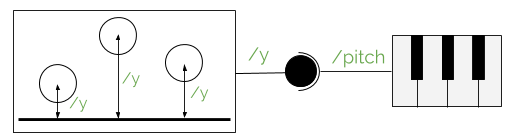
\includegraphics[keepaspectratio=true, width=\textwidth]{ModeleDeNotation/i/linkingParameters.png}
	\caption{Liaison de paramètres entre une partition et un synthétiseur}
	\label{fig:linkingParameters}
	\small
	\textit{ A gauche, une partition \textit{symbolist} constitué d'un trait horizontal et d'une suite de cercles placés plus ou moins haut selon l'axe vertical. A droite, un synthétiseur, pouvant représenté un objet (au sens instance de classe), une application, ou une machine indépendante. }
\end{figure}

Dans la figure \ref{fig:linkingParameters}, le formalisme graphique utilisé pour exprimer la connexion entre les paramètres de sortie de la partition et les paramètres d'entrée du synthétiseur est celui défini par UML 2.5.1 pour modéliser les architectures de composants \cite{omg2017}. En effet, il est pratique de considérer la partition et le synthétiseur comme deux composants logiciels pour étudier la connexion de leurs paramètres. Ici, le cercle noir attaché à la partition modélise un paramètre de sortie (\textit{interface fournie}, le message OSC \texttt{/y}), et l'arc de cercle attaché au synthétiseur représente un paramètre d'entrée (\textit{interface requise}, le message OSC \texttt{/pitch}).
Dans notre exemple, le synthétiseur a besoin de l'information \texttt{/pitch}, qui représente la hauteur du son à produire en Hertz, pour pouvoir fonctionner.
De fait, connecter le paramètre \texttt{/pitch} du synthétiseur au message \texttt{/y} envoyé par la partition lie les deux valeurs selon l'expression: $/pitch = f(/y(t))$
Soit, la hauteur du son produit par le synthétiseur est une fonction de la hauteur des cercles sur l'axe vertical évoluant au fil du temps. Cette connexion peut être effectuée de deux manières: 
\begin{enumerate}[label={(\arabic*)}]
	\item \textbf{Manuellement}: l'utilisateur devra alors connaître les paramètres d'entrée du synthétiseur et envoyé les messages correspondant en sortie lors de la lecture de la partition. Dans notre exemple, l'utilisateur devra explicitement créé un message \texttt{/pitch} pour chaque cercle de la partition et l'envoyer au synthétiseur.
	\item \textbf{(Semi-)Automatiquement}: Un protocole de communication peut être mis en place pour la connexion de \textit{symbolist} et du synthétiseur; le protocole mettra en relation les messages exposés par la partition \textit{symbolist} et les messages pouvant être reçus par le synthétiseur. Aussi, l'utilisateur devra s'assurer que les paramètres sont correctement liés, d'où le caractère semi-automatique de cette procédure. 
\end{enumerate}
%
Dans les deux cas, la fonction $f$ qui permettra, pour reprendre l'exemple, de lier la valeur de \texttt{/pitch} à \texttt{/y(t)} pourra être précisée en tirant profit des expressions \textit{odot} (voir section \ref{subsec:odotLibrary}).
Aussi, le protocole de communication devra s'assurer qu'une partition \textit{symbolist} est bien \textit{composable} avec le processus qu'elle veut contrôler. Entre autres, les interfaces exposées par l'un et l'autre doivent être compatibles \cite{chen2007}. Un des critères de la compatibilité peut simplement être la nécessité de mise en relation de paramètre du même type. Dans notre exemple, si \textit{/pitch} est de type \textit{float} et la valeur retournée par $f(/y(t))$ est une chaîne de caractères, alors la partition n'est pas composable avec le synthétiseur.

Pour réaliser cette fonctionnalité de connexion entre partition et processus de production sonore, deux technologies provenant du monde de l'informatique musicale possèdent un intérêt. La première technologie est le framework \textit{jamoma} qui permet l'encapsulation de patches Max\footnote{Pour rappel, un patch Max est une composition d'objets du langage de programmation visuelle Max. Les objets d'un patch Max sont reliés entre eux par des cordes, permettant leur communication par envoi de messages.} dans un module. Un module \textit{jamoma} déclare ses interfaces d'entrée et de sortie sous forme de liste de messages OSC, comme montré en figure \ref{fig:jamomaModule}.
\begin{figure}[H]
	\centering
	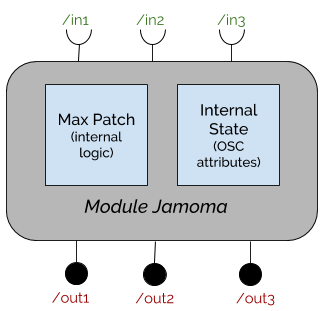
\includegraphics[keepaspectratio=true, width=0.5\textwidth]{ModeleDeNotation/i/jamomaModule.png}
	\caption{Structure d'un module jamoma}
	\label{fig:jamomaModule}
	\small
	\textit{ En haut, les connexions arc de cercle représentent l'interface d'entrée du module. En bas, les connexions en cercle rempli représentent l'interface de sortie du module.}
\end{figure}
Un module \textit{jamoma} maintient un état interne (\textit{internal state} sur la figure \ref{fig:jamomaModule}) reflétant la valeur courante des attributs exposés en entrée et en sortie du module.
La connexion entre les entrées et sorties du module et le patch Max encapsulé est définie à la création du module.
L'utilisation de modules \textit{jamoma} assure une communication basée sur l'envoi de messages au format OSC, ainsi qu'une exposition explicite des messages pouvant être envoyés et reçus par un module. 

La deuxième technologie digne d'intérêt est le protocole \textit{Minuit} qui décrit un système de requêtes entre processus utilisant le format OSC comme structure interne de données \cite{minuit2010}. \textit{Minuit} définit trois types de messages pouvant être envoyés: \texttt{get} permettant de lire la valeur d'un message OSC, \texttt{set} permettant d'écrire la valeur d'un message OSC, et \textit{listen} permettant de définir un écouteur sur une valeur de message OSC. Pour reprendre l'exemple cité plus haut, le protocole \textit{Minuit} permettrait à une partition \textit{symbolist} d'écrire ou de lire la valeur de l'attribut \textit{/pitch} du synthétiseur, ou bien permettrait au synthétiseur d'être tenu au courant de la valeur courante de \texttt{/y(t)}.

	
		
	\section{Abstraction des concepts de la notation traditionnelle}
	\label{sec:abstractionConcepts}
	L'application \textit{symbolist} veut s'abstraire du canevas de la notation traditionnelle, et même de tout autre système d'écriture préétabli, pour proposer aux compositeurs un environnement d'expression graphique libre, proche de l'usage du papier (voir section \ref{sec:geneseSymbolist}).
Cependant, ajouter certains concepts structurants au système de notation de \textit{symbolist} est un réel soutien à la pensée compositionnelle. A cet égard, deux concepts tirés de la CWMN, les concepts de \textit{staff} et de \textit{clef}, ont été intégrés à l'application. 
De plus, dans un souci d'exhaustivité et étant donné les pratiques de notation majoritairement utilisées par les compositeurs de musique contemporaine (voir annexe \ref{sec:analyseBesoins}, page~\pageref{sec:analyseBesoins}), les symboles de la CWMN ont été ajoutés à la palette \textit{symbolist} comme une contribution de ce stage.

\subsection{Concept de staff} 
\label{subsec:conceptDeStaff}
Le concept de \textit{staff} (\gls{portee} en anglais) a été défini et implémenté dans \textit{symbolist}.
Dans notre application, un \textit{staff} peut être représenté graphiquement par n'importe quel symbole qui sera alors considéré comme le symbole référent. Chaque symbole d'une partition \textit{symbolist} possède un message \texttt{/staff} dans le bundle OSC les décrivant. Par exemple, un symbole est attaché au staff d'identifiant 12 si son message \texttt{/staff} vaut 12.
Les symboles de la partition qui sont attachés à un \textit{staff} se voient attribuer une valeur temporelle de départ et de fin correspondant à leur point de départ et de fin vis à vis du symbole référent.
Le staff est une manière d'ordonner horizontalement (localement) les symboles d'une partition \textit{symbolist}. 
La figure \ref{fig:exempleDeStaff} montre un exemple de partition \textit{symbolist} composé d'un \textit{staff}, avec plusieurs symboles attachés, et de symboles libres.

\begin{figure}[H]
	\centering
	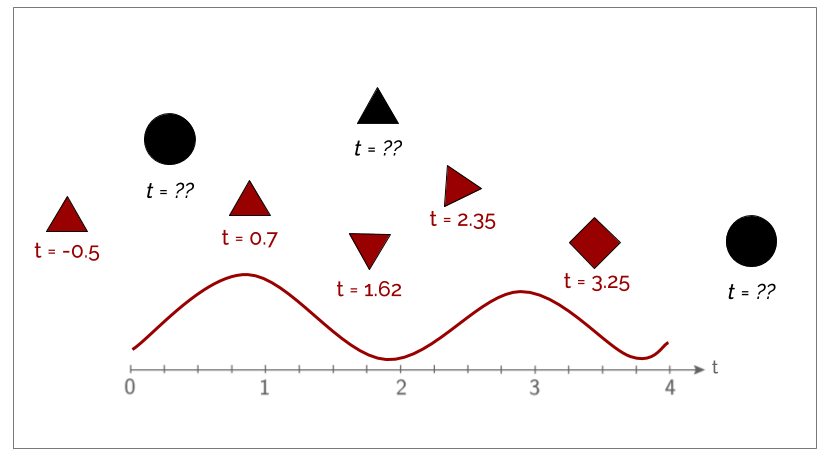
\includegraphics[keepaspectratio=true, width=0.8\textwidth]{ModeleDeNotation/i/staffConcept.png}
	\caption{Définition d'un staff dans une partition symbolist}
	\label{fig:exempleDeStaff}
	\small
	\it
	Le cadre représente une partition \emph{symbolist}. En rouge, le symbole référent du \emph{staff} (la courbe), et les symboles attachés au \emph{staff}. En noir, les symboles libres, sans positionnement temporel.
	Le temps de départ (position de l'extrémité gauche sur l'axe gradué) est donné pour chaque symbole attaché au staff et pour le symbole référent.
\end{figure}

Il est notable, dans la figure \ref{fig:exempleDeStaff}, qu'un symbole attaché à un staff n'est pas contraint de commencer dans l'intervalle temporel du symbole référent. Par exemple, le triangle placé à $t = -0.5$ est en dehors de l'intervalle temporel de la courbe qui commence à $t = 0$.

Comme vu en section \ref{sec:analyseSymbolist}, l'application \textit{symbolist}, dans sa version objet pour \textit{Max} et \textit{OpenMusic}, peut lancer une lecture temporelle de sa partition courante (grâce à l'envoi du message \texttt{time} dans Max, et à la barre de lecture intégrée dans \textit{OpenMusic}). A ce sujet, une lecture temporelle d'une partition \textit{symbolist} n'est possible que lorsqu'au moins un \textit{staff} a été défini. Dans le cas contraire, aucun intervalle temporel n'est présent dans la partition. Lorsque qu'un \textit{staff} a été créé et qu'une lecture temporelle est lancée, une barre de lecture apparaît dans l'interface \textit{symbolist}, accompagné de l'affichage du temps courant. La figure \ref{fig:readingTheScore} donne un exemple de lecture temporelle d'une partition \textit{symbolist}.

\begin{figure}[H]

\centering
\begin{minipage}{0.45\textwidth}
	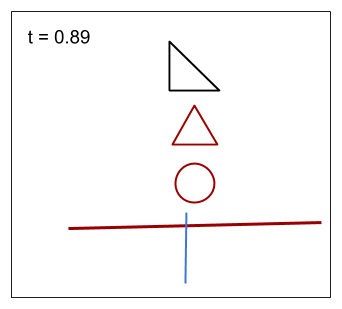
\includegraphics[keepaspectratio=true, width=0.8\textwidth]{ModeleDeNotation/i/readingTheScore.png}
\end{minipage}%
\begin{minipage}{0.45\textwidth}
\begin{lstlisting}[language = {C++}, numbers=none]
/staff/myStaff/voice/0/circle/1/name "myCircle"
/staff/myStaff/voice/0/circle/1/type "circle"
/staff/myStaff/voice/0/circle/1/x	40.6
[...]
/staff/myStaff/voice/1/triangle/1/name "myTriangle"
/staff/myStaff/voice/1/triangle/1/type "triangle"
/staff/myStaff/voice/1/triangle/1/x	40.5 
[...]
\end{lstlisting}
\end{minipage}%

\caption{Lecture temporelle d'une partition symbolist}
\label{fig:readingTheScore}
\small
\it
A gauche, une partition \emph{symbolist} entrain d'être lue: en bleu, la barre de lecture; en rouge, un staff avec deux symboles associés; en noir, un symbole libre. A droite, les informations envoyées en sortie par \emph{symbolist}, résultat de la lecture de la partition.
\end{figure}

La barre de lecture se déplace le long des symboles référents de chaque \textit{staff}. A chaque fois qu'elle rencontre un symbole associé au \textit{staff} courant, les informations du bundle OSC décrivant le symbole rencontré sont envoyées sur la sortie. Dans la figure \ref{fig:readingTheScore}, la barre de lecture a rencontrée deux symboles associés au \textit{staff} courant, leurs informations sont envoyées en sortie selon le formalisme suivant:
\begin{center}
\tiny 
/staff/<nom du staff>/voice/<numéro de la voix>/<id du symbole>/<nom d'attribut> <valeur de l'attribut>
\end{center}

Si les symboles associés à un même \textit{staff} se chevauchent, alors chaque symbole est considéré comme appartenant à une voix différente, se concrétisant par l'affichage d'un identifiant de voix différent dans les informations envoyées sur la sortie. La figure \ref{fig:readingTheScore} montre également qu'aucune information concernant le symbole libre n'est affichée. Aussi, la structure de \textit{staff} permet de séparer dans un partition les parties destinées à l'humain de celles destinées aux processus informatiques, recevant les bundles OSC.

A chaque nouveau \textit{staff} créé dans la partition, l'intervalle de temps est continué. La figure \ref{fig:stavesCreation} explicite le phénomène d'extension de l'intervalle temporel avec la création de nouveaux \textit{staff}.

\begin{figure}[H]
	\centering
	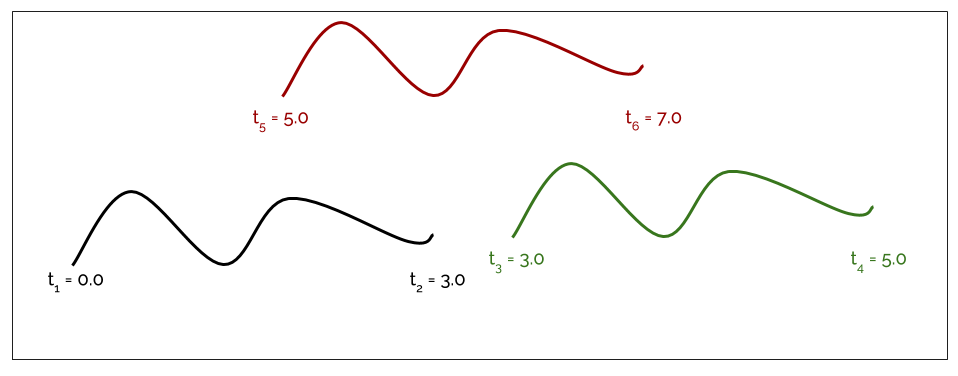
\includegraphics[keepaspectratio=true, width=0.9\textwidth]{ModeleDeNotation/i/stavesCreation.png}
	\caption{Extension de l'intervalle temporel de la partition}
	\label{fig:stavesCreation}
	\small
	\it
	En noir, le premier \emph{staff} créé définit un intervalle $[t_1, t_2]$ avec $t_1 = 0.0$ et $t_2 = 3.0$. En vert, le deuxième \emph{staff} créé définit un intervalle $[t_3, t_4]$ avec $t_3 = 3.0$ et $t_4 = 5.0$. En rouge, le troisième \emph{staff} créé définit un intervalle $[t_5, t_6]$ avec $t_5 = 5.0$ et $t_6 = 7.0$.
\end{figure}

Le placement des symboles référents de chaque \textit{staff} sur l'axe horizontal n'a pas d'incidence sur l'intervalle temporel définit; seul l'ordre de création compte. Aussi, dans la figure \ref{fig:stavesCreation}, le \textit{staff} rouge est placé avant le \textit{staff} vert sur l'axe horizontal, néanmoins il représente un intervalle temporel supérieur. 

\subsection{Concept de clef}
\label{subsec:conceptDeClef}
De fait, après avoir défini la sémantique du placement des symboles sur l'axe horizontal, la recherche de nouvelles fonctionnalités pour \textit{symbolist} a conduit à une réflexion sur la définition de la sémantique de l'axe vertical.
La CWMN (Common Western Music Notation) possède le concept de \textit{clef}, qui est un symbole placé au début d'une portée, associant à chaque ligne de la portée une hauteur représentée par un nom de note\footnote{Dans la CWMN, la hauteur d'un son est défini par un nom de note et un numéro. Par exemple, un son de fréquence 440Hz correspond au couple nom-numéro $(la, 3)$. Néanmoins, par convention, le numéro des notes est omis lors de la lecture d'une partition.}.
Aussi, les notes portent le nom de la ligne sur laquelle elles se trouvent.
La figure montre un exemple de changement de clef sur une même portée qui a pour conséquence de changer le nom des notes placées à la suite.
\begin{figure}[H]
	\centering
	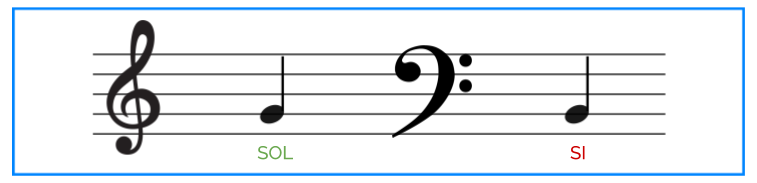
\includegraphics[keepaspectratio=true, width=0.6\textwidth]{ModeleDeNotation/i/clefsCWMN.png}
	\caption{Conséquence du changement de clefs sur le nom des notes}
	\label{fig:clefsCWMN}
	\small
	\textit{A gauche, le symbole de la clef de sol suivi d'une note placée sur la deuxième ligne de la portée. A droite, le symbole de la clef de fa suivi d'une note placée sur la deuxième ligne de la portée.}
\end{figure}
Si une clef de sol est inscrite sur la portée alors toutes les notes se trouvant à la suite sur la deuxième ligne de la portée auront pour nom \textit{sol}. Si une clef de fa est inscrite sur la portée alors toutes les notes se trouvant à la suite sur la deuxième ligne de la portée auront pour nom \textit{si}.

En s'inspirant de la CWMN, le concept de clef a été défini pour l'application \textit{symbolist}, bien qu'il ne soit pas à ce jour implémenté. Comme pour la CWMN, une clef est associé à un \textit{staff} dans \textit{symbolist}. En tirant profit du langage \textit{o.expr} (voir section \ref{subsec:odotLibrary}), une clef est définie dans \textit{symbolist} comme une liste d'expressions \textit{odot} s'appliquant à l'ensemble des symboles associés à un \textit{staff}.
 Par exemple, une clef peut déterminer l'ordre vertical des symboles attachés à un \textit{staff} comme étant la fonction inverse du message \textit{/pitch}. Dans ce cas, la clef contiendra l'expression  /y $= 1 /$ /pitch.

Pour expliciter la transformation des symboles associés à un \textit{staff} par application d'une clef, la procédure \ref{alg:applyKey} est présentée.

\begin{procedure}[H]
	\caption{ApplyKey($staff$, $clef$)}
	\label{alg:applyKey}
    
    \SetKwFunction{applyExpr}{ApplyExpr}
    
     
	\KwData{$staff$ une liste de symboles, représentant l'ensemble des symboles attachés au staff pour lequel la clef va être appliquée.}
	\KwData{$clef$ liste d'expressions \textit{odot}}
    \KwResult{L'ensemble des expressions \textit{odot} contenues dans la clef sont appliquées aux symboles du $staff$}
	
    \DontPrintSemicolon
    \BlankLine
    
	\ForEach {$expr$ t.q $expr \in clef$}{
    	\ForEach {$symbol$ t.q $symbol \in staff$}{
    		\applyExpr{$expr$, $symbol$}\;
    	}
    }    
	
\end{procedure}


\subsection{Intégration des symboles de la CWMN}
\label{integrationCWMN}
L'intégration des symboles de la CWMN est une des contributions de ce stage à l'application \textit{symbolist}.
Une analyse des besoins des compositeurs en terme d'outils de notation musicale a été menée et est présentée en annexe \ref{sec:analyseBesoins} page~\pageref{sec:analyseBesoins}. Cette analyse se présente sous la forme d'un questionnaire sur les pratiques de notation des compositeurs. A la question \og Pouvez-vous décrire votre worflow de notation? \fg, la quasi-majorité des compositeurs ont dit utiliser les outils de notation orientés CWMN dans leur phase de travail. Ce constat a donc motivé la volonté d'intégration de la CWMN dans la palette de symboles de l'application \textit{symbolist}.

Les logiciels performants pour l'édition de partitions en CWMN sont nombreux. symbolist ne prétend pas les concurrencer. De plus, les règles de mise en page d'une partition en CWMN sont pléthore et complexes. Par exemple, les techniques pour la justification horizontale des notes sur une portée est un sujet très discuté \cite{blostein1991}. Aussi, pour rester dans la philosophie de \textit{symbolist} qui est celle du dessin libre, les symboles de la CWMN ont été simplement mis à disposition dans la palette. Par la suite, l'implémentation des règles de mise en page de la notation traditionnelle sera à considérer.

Il existe une forte corrélation entre l'écriture textuelle et l'écriture musicale. Aussi, de multiple polices de caractères existent pour le texte, et il en est de même pour les polices de caractères musicaux.
Pour implanter les symboles de la CWMN dans \textit{symbolist}, la police de caractères \textit{open source} SMuFL (\textit{Standard Music Font Layout}) \cite{smufl2016}. Plus précisément, SMuFL est une spécification pour la création d'une police de caractères musicaux, maintenant soutenue par le groupe W3C Music Notation Community Group. SMuFL définit un dictionnaire de symboles musicaux (appelés des glyphes pour une police de caractères) chacun identifié par un numéro de caractère Unicode. SMuFL définit également les règles régissant la forme, la taille et la composition des caractères musicaux, et met à disposition de l'utilisateur l'ensemble de ces métadonnées dans des fichiers au format JSON.

La police de caractères \textit{Bravura}, qui est une implémentation de SMuFL, a été utilisée pour \textit{symbolist}. \textit{Bravura} est la police de caractères intégrée au logiciel de notation \textit{Dorico} développé par l'entreprise \textit{Steinberg}.
La figure donne un exemple de composition effectuée dans \textit{symbolist}, où les symboles de la police \textit{Bravura} sont mis à profit.

\begin{figure}[H]
	\centering
	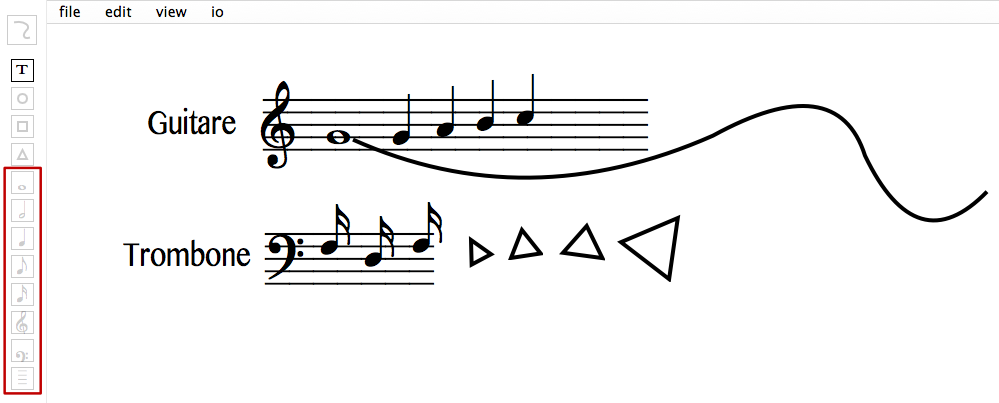
\includegraphics[keepaspectratio=true, width=\textwidth]{ModeleDeNotation/i/bravuraCreation.png}
	\caption{Composition graphique avec les caractères de la police Bravura}
	\label{fig:bravuraCreation}
	\small
	\it
	En \textcolor{red}{rouge}, quelques glyphes de la police \emph{Bravura} ajoutés à la palette de \emph{symbolist}.
\end{figure}
     


	
%%%%% CONCLUSION %%%%%
\clearpage
\chapter{Conclusion}
Comme peut en témoigner l'Histoire, la notation musicale n'est pas un processus monolithique. L'écriture de la musique est influencée par le contexte technologique propre à chaque époque. Aussi, la musique contemporaine, qui s'installe à partir des années 50, voit ses pratiques profondément impactées par l'usage de l'électronique et l'informatique. Aujourd'hui encore, l'apparition de nouvelles technologies (machine learning, réalité virtuelle, IoT\footnote{Internet of Things}…) pousse les compositeurs à réinventer leur relation avec la musique et la manière de la noter. Au-delà de la musique contemporaine, la composition multimédia, tirant profit de la profusion des supports technologiques de notre époque (vidéo, audio, capteurs, actionneurs…), cherche encore un système de notation qui lui serait adéquat. Au moment de la rédaction de cette étude, les technologies pour la création musicale sont trop récentes et trop nombreuses pour pouvoir proposer une pratique notationnelle unique. De fait, chaque compositeur a ses propres besoins en termes d'écriture, ce qui devrait pousser les outils informatiques à proposer plus de fonctionnalités permettant l'invention d'une notation par l'utilisateur.

Or, les logiciels actuels de notation musicale ne répondent qu'en partie à la prérogative d'extensibilité ou de renouveau des pratiques d'écriture de la musique, dans le but de s'accorder avec la création contemporaine. Une première catégorie des logiciels existants intègre bien la notation traditionnelle mais ne fournit que peu de moyens pour l'étendre et l'adapter à l'écriture d'œuvres nouvelles. Une deuxième catégorie de logiciels approche la transcription musicale sous l'angle des pièces électroacoustiques et multimédias, en incorporant aux partitions une dimension interactive. Cependant, cette seconde catégorie délaisse quelque peu l'expressivité symbolique au profit de la description temporelle des processus régissant les œuvres.

Dans ce contexte, le développement du logiciel \textit{symbolist} a été initié afin d'adresser le problème du manque d'outils permettant de transcrire symboliquement les œuvres contemporaines \cite{gottfried2018}.
\textit{symbolist} est un éditeur graphique libre où le compositeur peut créer à volonté tous types de symboles et les enregistrer dans une palette. Ce logiciel est destiné à être encapsulé dans les environnements \textit{OpenMusic} et \textit{Max}, et utilise le protocole OSC pour s'interfacer avec l'extérieur.
La poursuite du développement de \textit{symbolist} constitue le cadre du présent stage. Aussi, la génèse et les caractéristiques du logiciel seront explicitées dans le rapport final d'activités.
Dans la continuité de la période d'étude bibliographique, un recueil du besoin sera effectué auprès des compositeurs de musique contemporaine (de l'IRCAM et d'ailleurs), afin de déterminer précisément les attentes des utilisateurs potentiels de \textit{symbolist}.
De plus, une démarche d'analyse et de rétro-ingénierie sera menée sur le logiciel, étant donné son état avancé de développement.
Enfin, une étape d'organisation et de planification des méthodes de travail sera préalable à l'implémentation de nouvelles fonctionnalités.   
 

%%%%% BIBLIOGRAPHIE %%%%%
\printbibliography

%%%%% TABLE DES FIGURES %%%%%
\listoffigures

%%%%% GLOSSAIRE %%%%%
\printglossary

%%%%% ANNEXES %%%%%
\appendix
\chapter{Annexes}
% Pour faire une référence d'une annexe
% (Annexe \ref{sec:nomsection} page~\pageref{sec:nomsection})
\section{Analyse des besoins pour la notation de la musique contemporaine et la composition multimédia}
\label{sec:analyseBesoins}

L'étude bibliographique, amorcée en amont du stage, a permis de dresser un état des lieux des outils pour la notation musicale. Cependant, les besoins réels en termes de notation doivent être recueillis auprès des principaux intéressés: les compositeurs. Aussi, la démarche de recueil tente de répondre à plusieurs questions: Est-il possible de déterminer un noyau commun adressable des besoins de notation des compositeurs? Ou alors, leurs besoins sont-ils spécifiques à chacun d'eux, ce allant dans le sens d'une notation musicale créée et adaptée à chaque compositeur et à chaque pièce \cite{bosseur2005}?

A l'initiative de Jean Bresson, le groupe de travail \textit{notation} a été lancé à l'Ircam. Ce groupe rassemble des chercheurs, des compositeurs ou encore des réalisateurs\footnote{Un réalisateur en informatique musicale travaille de pair avec un compositeur de musique contemporaine, pour réaliser techniquement les pièces musicales imaginées par le compositeur.} en informatique musicale. Le groupe de travail s'organise autour de discussions, de débats ou de présentations sur le sujet de la notation musicale en musique contemporaine. Aussi, c'est lors de ces séances que l'idée de la création d'un questionnaire pour le recueil des besoins des compositeurs a émergée.
Le questionnaire établi comporte trois questions à réponse ouverte; il a été rendu au plus court dans le but de recevoir le plus de réponses possibles. Les trois questions sont les suivantes
\begin{enumerate}[label={(\arabic*)}]
	\item \textit{Pouvez-vous décrire votre workflow de notation?}: quelles sont les pratiques notationnelles des compositeurs, et les outils qu'ils utilisent.
	\item \textit{Pouvez-vous nommer trois fonctionnalités que vous jugez primordiales dans un logiciel de notation musicale?}: isolement de préoccupations principales des compositeurs en termes de notation.
	\item \textit{Concernant les outils de notation que vous utilisez, y a-t-il des problèmes que vous voudriez adresser?}: problématiques rencontrées par les compositeurs, et leur sentiment général par rapport à leurs outils.  
\end{enumerate}

Le questionnaire a été envoyé à plus de trois cents compositeurs par mail, en tirant profit des listes de diffusion de l'Ircam.
Quinze compositeurs ont répondu, ce qui permet déjà d'analyser et de tirer des motifs de leurs retours. Les résultats pour chaque question sont présentées et analysées ci-après.

\paragraph{Pouvez-vous décrire votre workflow de notation?} Cette première question visait à déterminer quels outils de notation sont utilisés par les compositeurs et dans quelles proportions. Le tableau \ref{tab:workflowNotation} présente tous les types d'outils de notation cités dans les réponses, et pour chacun d'eux le nombre de compositeurs en faisant usage sur les quinze ayant répondu.

\newcolumntype{C}{>{\centering\arraybackslash} X}
\begin{table}[H]
	
    \renewcommand{\arraystretch}{1.5}
    \centering
    
	\begin{tabularx}{\textwidth}{|C|C|C|C|C|}
	\hline
    Papier & Logiciels orientés CWMN & Logiciels orientés électroacoustiques & Logiciels de design graphique (\textit{Adobe Illustrator}, \textit{INKScape}) & Logiciels mixtes (\textit{INScore}) \\
    \hline
    10/15 & 11/15 & 5/15 & 3/15 & 1/15 \\
    \hline
	\end{tabularx}
	
   	\caption{Sondage sur l'utilisation des outils de notation musicale}
    \label{tab:workflowNotation}
	\small
	\textit{Il est a noté que le nombre d'outils utilisés par chaque compositeur variant, le nombre total de réponses n'est pas égal à quinze.}
\end{table}

Les résultats du tableau \ref{tab:workflowNotation} montre que le papier et les logiciels de notation utilisant le système traditionnel occidental sont les plus utilisés par les compositeurs. En effet, le support papier est souvent utilisé par les compositeurs au début de leur phase de composition, pour ne pas brider leur créativité en s'imposant le canevas d'un logiciel. De même, la forte utilisation des programmes de notation orientés CWMN (\textit{Sibelius}, \textit{Finale}, \textit{MuseScore}, etc.) s'explique par la grande diffusion de ces outils sur le marché international, alors que les outils pour la notation de l'électroacoustique relève d'une utilisation plus discrète, touchant en majorité les milieux de la recherche en informatique musicale.
Également à noter, quelques compositeurs (trois parmi quinze) décrivent les stations audionumériques qu'ils utilisent comme de véritables outils de notation de la musique; cela amène à reconsidérer le statut de ces logiciels (voir la discussion de la section \ref{sec:notationMusiqueContemporaine}).

\paragraph{Pouvez-vous nommer trois fonctionnalités que vous jugez primordiales dans un logiciel de notation musicale?} La deuxième question avait pour but de profiler un noyau de caractéristiques dont l'absence dans un outil de notation serait rédhibitoire pour la communauté des compositeurs de musique contemporaine.
Voici la liste des propositions faites par les compositeurs, dans l'ordre de la plus citée à la moins citée:
\begin{itemize}[label=--]
	\item Liberté (flexibilité) dans la composition graphique des partitions (7/11)
	\item Automatisation du rendu graphique (alignement, mise en page…) (6/11)
	\item Rendu audio de la partition (6/11)
	\item Intégration de la CWMN (4/11)
	\item Interopérabilité (4/11)
	\item Visualisation de formes d'ondes, et spectres (3/11)
	\item Symboles de spatialisation (1/11)
\end{itemize}

Seuls onze compositeurs ont bien répondu à cette question, ce qui explique le changement de mesure. Les résultats montrent l'intérêt des compositeurs quant à la liberté d'expression graphique procurée par les logiciels de notation. La qualité de rendu graphique des partitions et l'aisance d'utilisation d'un logiciel est également un impératif. Aussi, les compositeurs réclament une logique de mise en page efficace, pour traiter, par exemple, l'alignement ou l'espacement des éléments graphiques entre eux.
Il est à noter que l'intégration des symboles du système traditionnel occidental n'est pas considéré comme primordial. D'ailleurs, la capacité de connecter un logiciel de notation musicale à d'autres systèmes de production sonore est une considération de même niveau pour les compositeurs. L'impératif d'interopérabilité est liée à l'impératif de rendu audio de la partition (le rendu effectué par les logiciels de synthèse sonore).

\paragraph{Concernant les outils de notation que vous utilisez, y a-t-il des problèmes que vous voudriez adresser?} La dernière question a été formulée pour identifier les faiblesses des outils de notation ou les difficultés qu'ils induisent dans le processus de composition.  Les problèmes identifiés sont les suivants:
\begin{itemize}[label=--]
	\item Mauvais alignement des éléments évoluant à des temporalités différents: par exemple, alignement des éléments de deux portées ayant des signatures rythmiques différentes.
	\item Mauvais alignement des éléments relevant de paradigmes différents: par exemple, alignement d'une forme d'ondes et de notes de musique.
	\item Peu de liberté pour la composition et le dessin graphique.
	\item Pas de vues multiples d'une même partition dans un même logiciel de notation. Le compositeur est alors obligé de répliquer sa partition dans plusieurs logiciels, chacun lui offrant une vue précise de sa partition.
\end{itemize}

La plupart des plaintes recueillies concernent la capacité d'expression et le rendu graphique des logiciels; cela va de pair avec la considération de ces fonctionnalités comme étant primordiales pour un programme de notation musicale.
\clearpage

% Appendix declaration with a 90° rotated figure
\rotatebox{90}{
	\begin{minipage}{0.90\textheight}
		\section{Modèle de l'application symbolist}
		\label{sec:symbolistModelClassDiagram}
		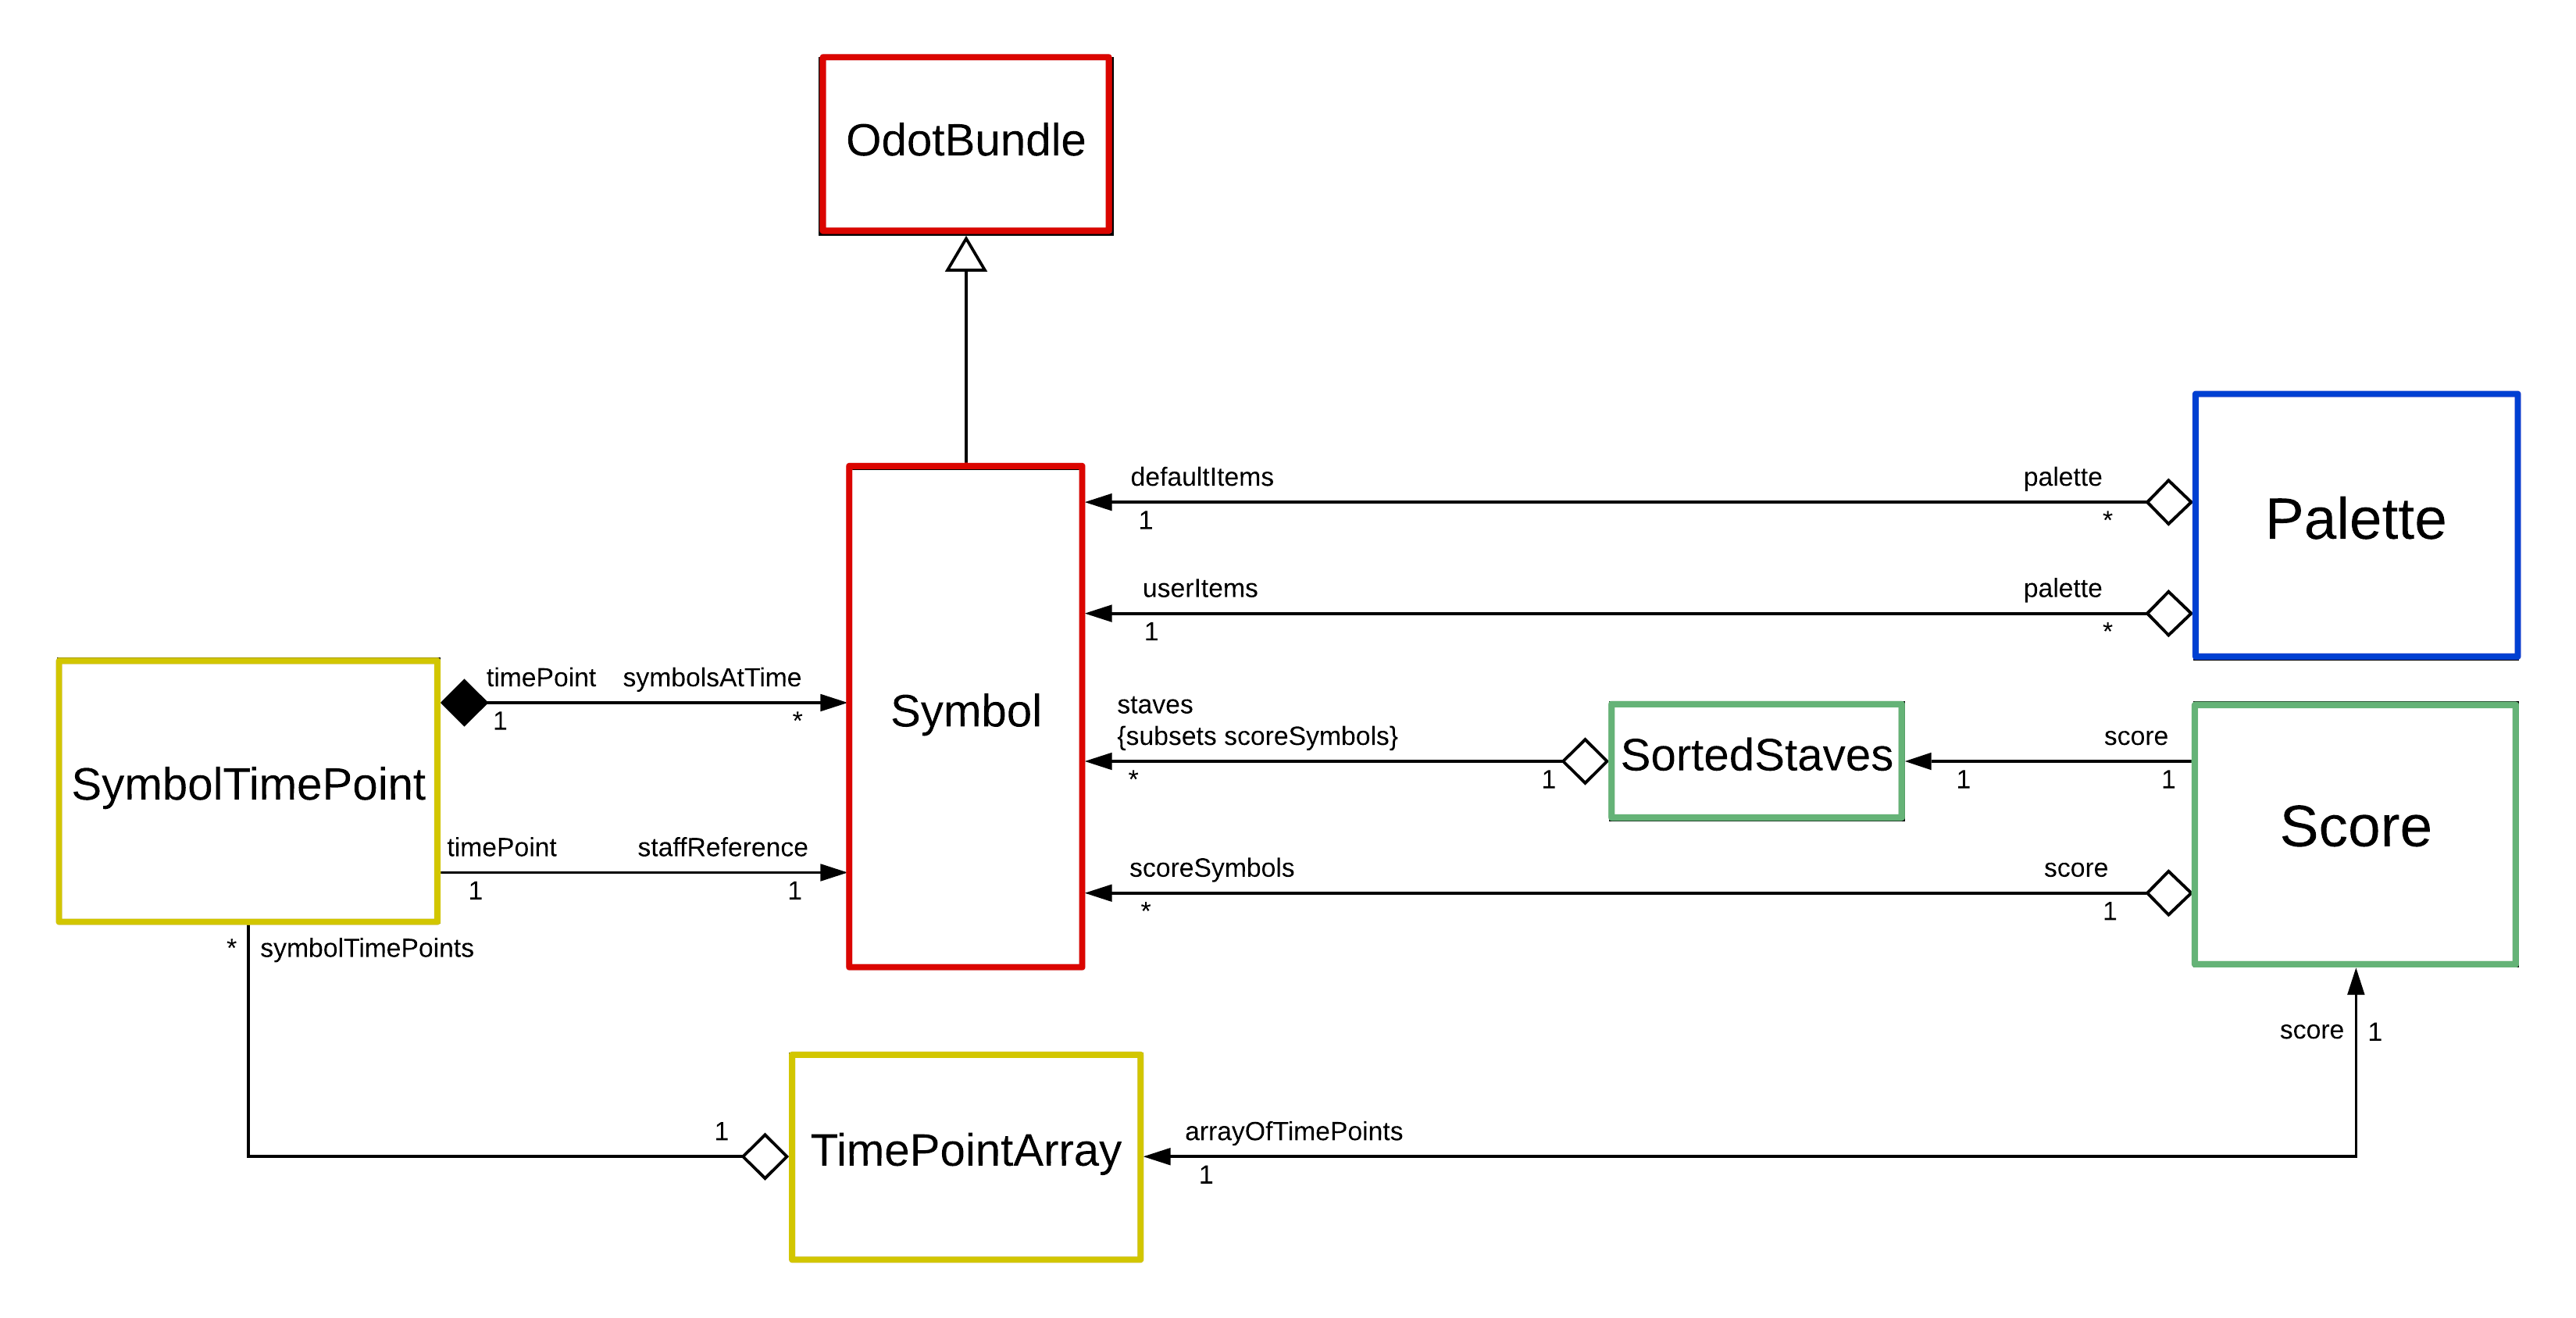
\includegraphics[keepaspectratio=true, width=\textwidth]{Annexes/i/symbolistModelClassDiagram.png}
		\captionof{figure}{Diagramme de classes pour le modèle de l'application symbolist}
		\label{fig:symbolistModelClassDiagram}	
		\medskip
		\small
		\it
		En \textcolor{red}{rouge}, la classe \emph{OdotBundle}, qui encapsule la structure d'un bundle \emph{OSC}, et la classe \emph{Symbol} dont les instances représentent les symboles de la partition. Chaque symbole de la partition possède une structure de bundle OSC, d'où la relation d'héritage entre la classe \emph{OdotBundle} et \emph{Symbol}.
		En \textcolor{blue}{bleu}, la classe \emph{Palette}, regroupant les symboles pouvant être dessinés sur la partition, qu'ils aient été définis par l'utilisateur ou existaient par défaut dans l'application.
		En \textcolor{green}{vert}, les classes \emph{Score} et \emph{SortedStaves} décrivant les symboles présent dans la partition.
		En \textcolor{yellow}{jaune}, les classes \emph{SymbolTimePoint} et \emph{TimePointArray} définissant la logique d'ordonnancement temporel des symboles associés à un \emph{staff}.  
	\end{minipage}
}
\clearpage

\rotatebox{90}{
	\begin{minipage}{0.85\textheight}
		\section{Architecture finale de l'application symbolist}
		\label{sec:symbolistFinalStructure}
		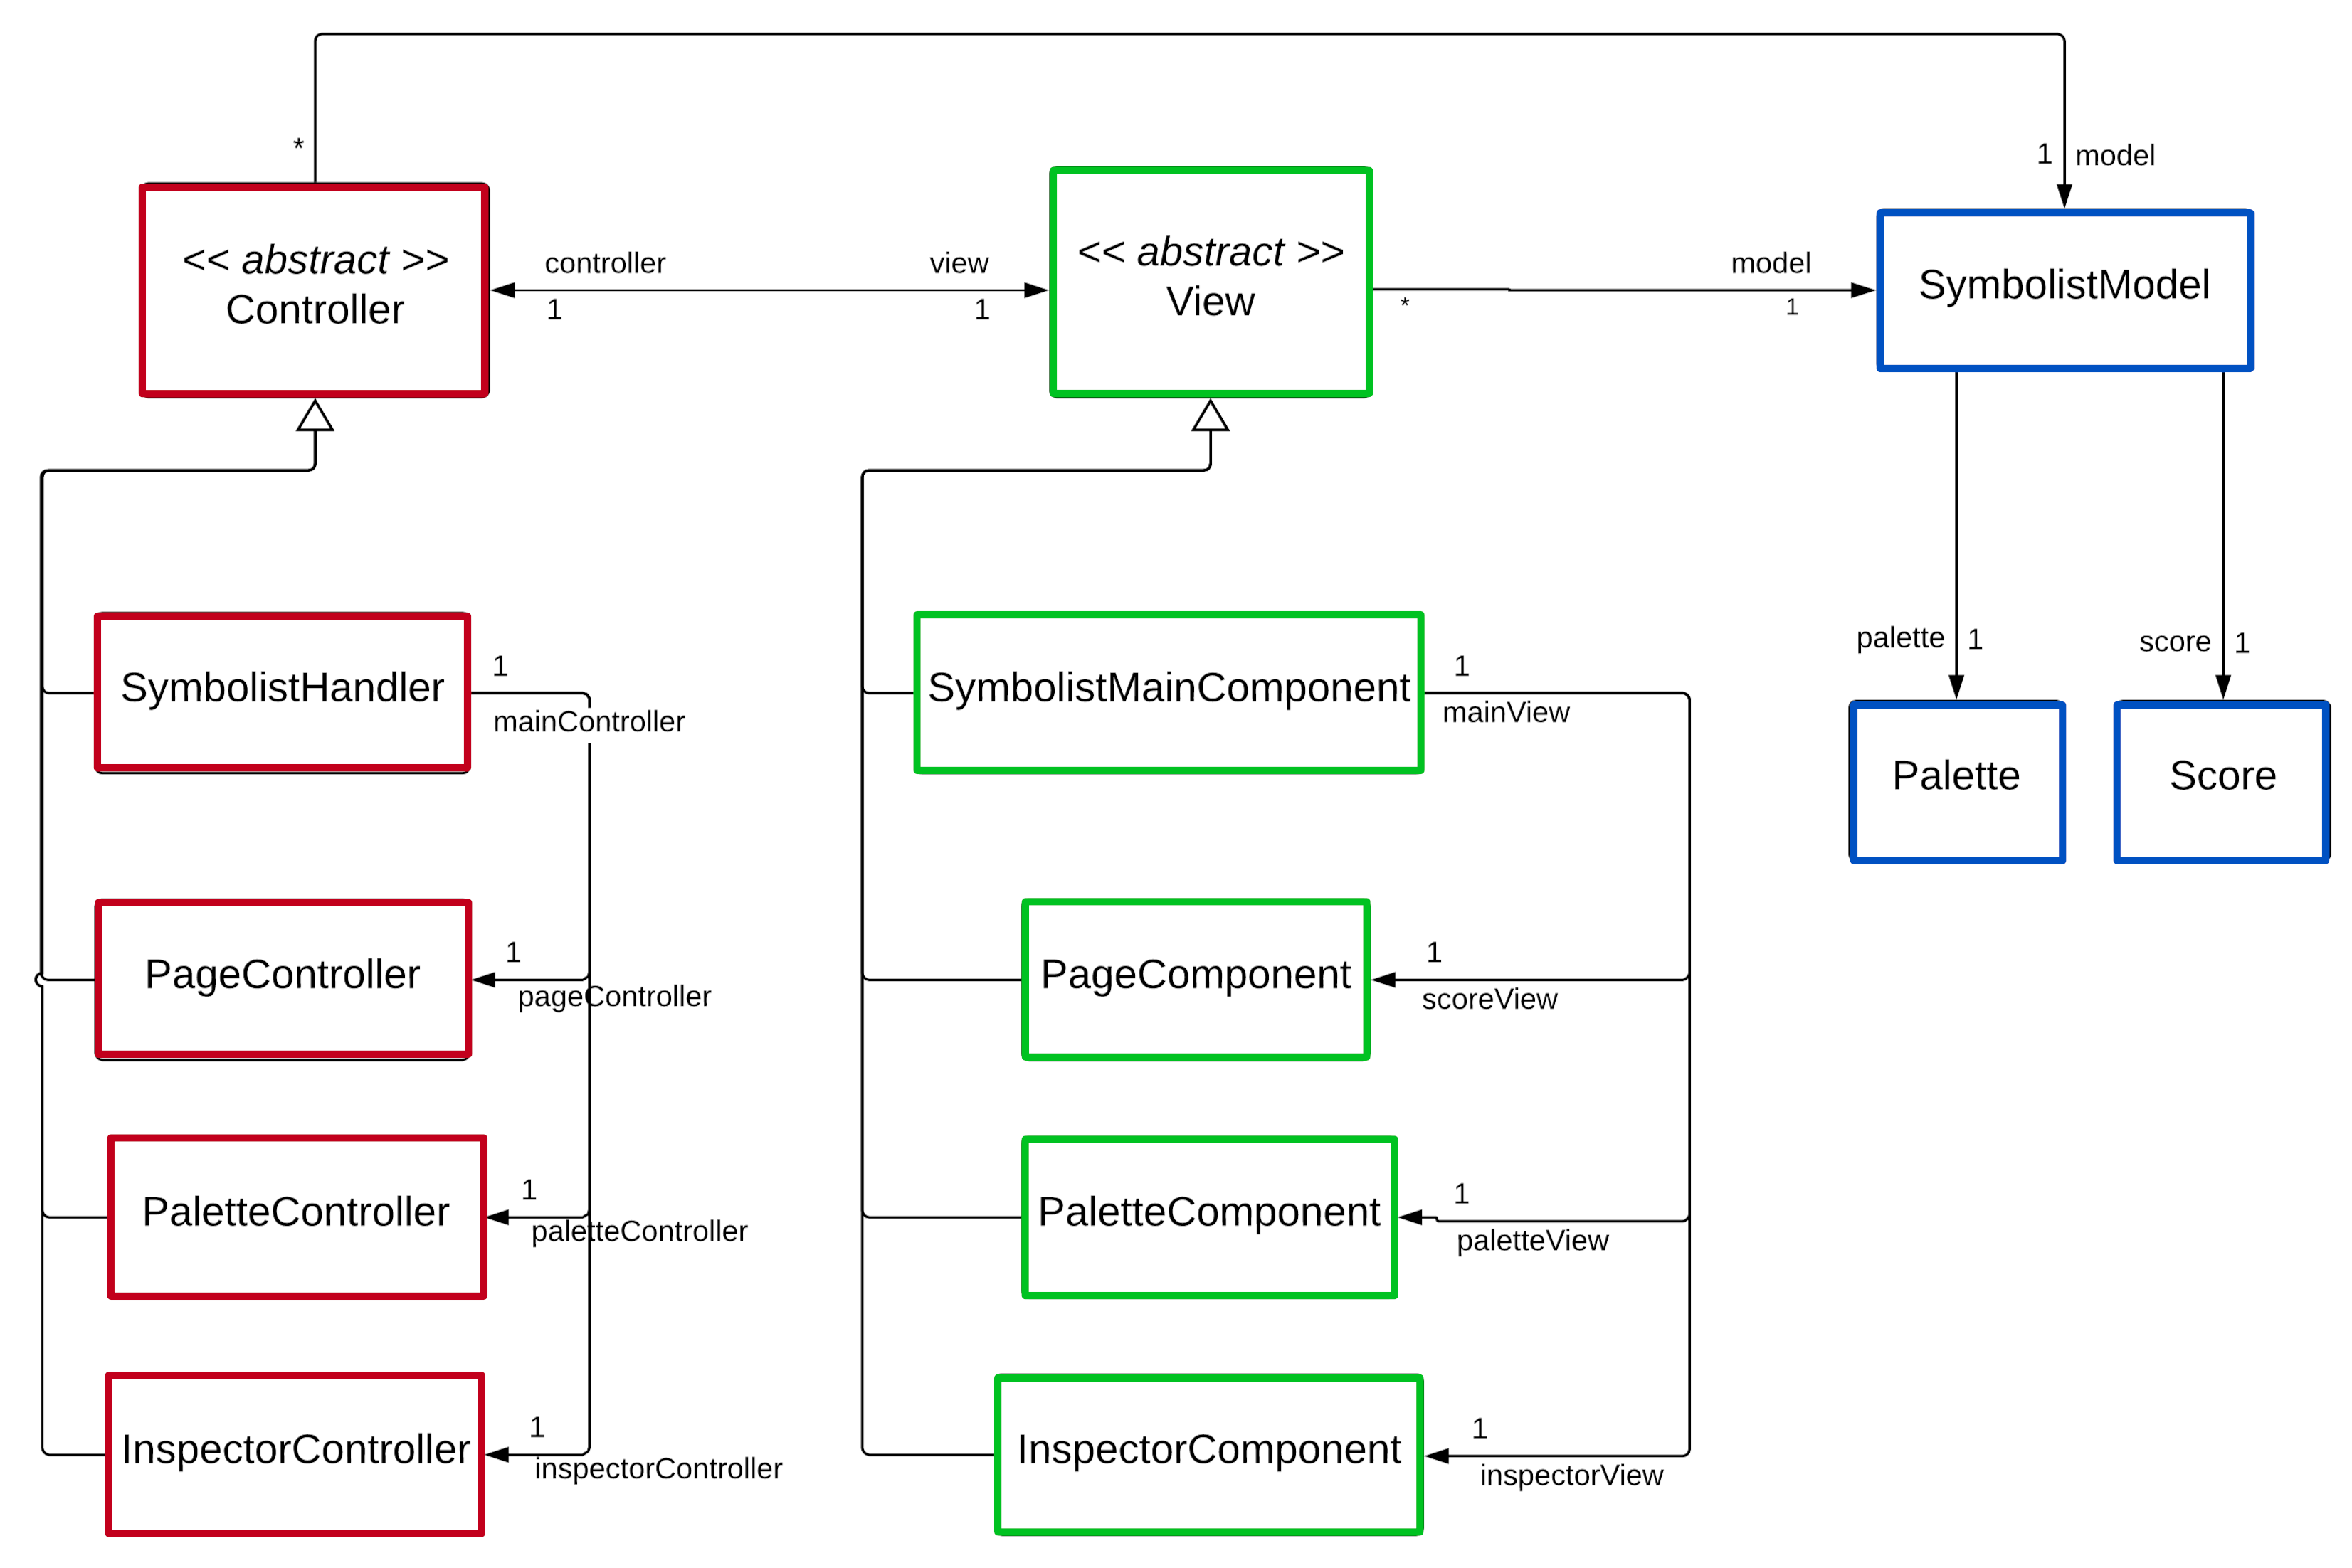
\includegraphics[keepaspectratio=true, width=\textwidth]{Annexes/i/symbolistFinalStructure.png}
		\captionof{figure}{Diagramme de classes présentant l'architecture de l'application symbolist après restructuration}
		\label{fig:symbolistFinalStructure}	
		\medskip
		\small
		\it
		En \textcolor{red}{rouge}, .
		En \textcolor{blue}{bleu}, .
		En \textcolor{green}{vert}, .  
	\end{minipage}
}
\clearpage


\end{document}
     
